\documentclass[english]{ifacconf}
\usepackage[utf8]{inputenc}
\usepackage{array}
\usepackage{float}
\usepackage{amsmath}
\usepackage{amssymb}
\usepackage{graphicx}
\usepackage{natbib}
\usepackage{enumitem}

\begin{document}
\begin{frontmatter}
	
\title{Shared Control Between Adaptive Autopilots and Human Operators for Anomaly Mitigation}

\thanks[footnoteinfo]{This work was supported by the Boeing Strategic University Initiative.}

\author[MIT]{Benjamin T. Thomsen} 
\author[MIT]{Anuradha M. Annaswamy} 
\author[Boeing]{Eugene Lavretsky} 

\address[MIT]{Massachusetts Institute of Technology, 
   Cambridge, MA 02139}%\\email: [thomsen, aanna]@mit.edu}
\address[Boeing]{The Boeing Company, 
   Huntington Beach, CA 92647}

\begin{abstract}
%This paper outlines a shared decision-making and control framework between adaptive controllers and human supervisors, able to recover control performance following anomalous changes in plant dynamics. Model reference adaptive control relies on accurate understanding of plant dynamics to guarantee stability and performance, and these guarantees are lost when severe anomalies introduce unexpected and unmodeled dynamics to the plant. We introduce a shared control architecture in which a human supervisor diagnoses anomalous closed-loop dynamic behavior and makes suitable changes to the control model of the system in order to recover nominal performance. This shared response allows for continued autonomous adaptive control without transferring control responsibilities to the human operator. Anomaly response with shared control is demonstrated on an unmanned very flexible aircraft (VFA) platform, whose actuators suddenly change from first-order to second-order.
%Changes to plant dynamics during operation, whether controlled manually by a human or autonomously by model-based control algorithms, can lead to instability and failure. 
%The control of plants having anomalous dynamics is difficult for both human operators and autonomous model-based control algorithms. We introduce a shared decision-making and control framework based on adaptive control which gives supervisory human operators a targeted responsibility in the mitigation of dynamical anomalies and enables the recovery of closed-loop system stability and command tracking performance without transferring control responsibilities to the human operator. Anomaly response with shared control is demonstrated on an unmanned aerial vehicle, whose actuators suddenly change from first-order to second-order.
As aerial vehicles become more autonomous, and guidance and navigation systems become increasingly network-centric, there is a need to consider a swift response to the growing forms of anomalies that may occur in these systems. We introduce a shared decision-making and control framework between a human operator and an adaptive autopilot, where the human operator plays a supervisory role and the adaptive autopilot retains the responsibility for low-level regulation and command tracking tasks. The human operator provides key inputs based on a higher-level perception of the anomaly, such as an increased lag in response to command inputs, which are then used by the adaptive autopilot in a suitable manner. The resulting shared control architecture is demonstrated on an unmanned aerial vehicle, whose actuators suddenly change from first-order to second-order due to an anomaly.
\end{abstract}
\begin{keyword}
adaptive control, output feedback, anomaly detection and recovery, high relative degree, shared control
\end{keyword}

\end{frontmatter}

\section{Introduction}
%Adaptive control and modeling assumptions.
%Model-based feedback control designs, based on \textit{a priori} knowledge of system dynamics, are ubiquitous in industries such as aerospace, as they provide the ability to specify characteristics of the closed-loop system dynamics, and ensure stability, optimality, and robustness over a range of operating conditions. The field of adaptive control addresses a limitation of control based on models of plant dynamics, namely that parameters used to model the plant may be uncertain. Model reference adaptive control (MRAC), as described by \cite{narendra2012stable}, accommodates these parametric uncertainties through online tuning of control parameters to ensure specified closed-loop dynamics are realized. 
In flight control systems, as in any complex dynamic system, uncertainties are inevitable. Uncertainties may occur for myriad reasons including modeling errors, environmental variations, unforeseen anomalies and disturbances, and of late, cyber attacks. The field of adaptive control (\cite{narendra2012stable, lavretsky2013robust}) addresses a class of such uncertainties which are due to unknown parameters. By changing the control parameters online using a suitably constructed tracking error, the adaptive controller self-tunes its parameters and compensates for parametric uncertainties using online measurements. Recent advances in MRAC have included the development of closed-loop reference models (CRMs) by \cite{gibson2013adaptive}, which greatly improves transient performance during online learning. While adaptive control is able to guarantee stability and tracking convergence in the presence of parametric uncertainties, other properties of the system -- such as the order of a linear system -- are assumed to be known \textit{a priori} for control design. 
%In practice, dynamical behavior is excluded from the control model for simplicity and ease of analysis if it sufficiently fast relative to the closed-loop system bandwidth.

%Human pilots and operators, and their struggles with unfamiliar, off-nominal dynamics. %Remote human pilots and further difficulties
Human operators of dynamical systems also develop mental models of expected plant behavior, often over long periods of active learning. Human pilots, for example, have been modeled and studied extensively to examine their use of information feedback and ability to adapt their control strategies to unfamiliar situations (see, for example, \cite{mcruer1967review, phatak1969model, hess2015modeling, zaal2016manual}). In stressful situations, human pilots tend to apply high control gains, which coupled with certain dynamical anomalies may lead to pilot-induced oscillations and an increased risk of loss of control (\cite{hess1997unified}). \cite{belcastro2014preliminary} found that the majority of transport aircraft loss of control incidents over a 15-year period involved inaction or improper action by the flight crew. \cite{endsley1996automation} points to pilot error following a transition from autonomous to manual control (often as the result of an anomaly) as a common factor in loss of control incidents. Issues with manual control of dynamical systems are exacerbated when the human operator is physically separated from the dynamics of the system, as is the case with remotely piloted vehicles (\cite{mccarley2004human, tvaryanas2008recurrent}). The additional complexities involved with remote operation include a lack of sensory and perceptive cues regarding the plant state and its environment, time delays between the plant and operator for both sensing and actuation, and difficulty ascertaining the open-loop dynamical response between control input and plant output (\cite{lam2008haptic}). The question then is whether one can combine both an adaptive control methodology and a remote human supervisor's decision-making and their complementary merits and mitigate the effects of severe anomalies in a more efficient manner. The design of such a shared control is the focus of this paper.

The results of this paper build on our earlier work on shared control architectures of adaptive autopilots and human pilots, reported in \cite{farjadian2017bumpless} and \cite{thomsen2018shared}. Unlike these two papers, our focus here is on the case when only partial states are available as output measurements. In Section \ref{sec:problem}, the control problem investigated in this paper is described. Our explicit shared control solution to this problem is described in Section \ref{sec:shared_ctrl}. The shared decision-making and control framework is applied to the longitudinal control of high altitude, long endurance (HALE) unmanned aerial vehicles (UAVs) and simulated numerically in Section \ref{sec:vfa}. We summarize the work in Section \ref{sec:summary}.

\section{Problem Statement}\label{sec:problem}
%Control of plant with unknown/uncertain parameters. 
We consider linear multi-input multi-output (MIMO) plant models of the form
\begin{equation}
\begin{gathered}
\dot x_p = (A_p + B_p \Theta_p^T) x_p + B_p \Lambda_p u_p \\
y_p = C_p x_p, \qquad z_p = C_{pz} x_p \label{eq:plant_dynamics}
\end{gathered}
\end{equation}
where $x_p$ is the plant state, $u_p$ is the plant input, $y_p$ is measured output, and $z_p$ is regulated output. Uncertain dynamics lead to the introduction of unknown $\Theta_p$ and $\Lambda_p$ in the plant model. It is assumed that the matrix $CB$ has full rank, and thus the plant has uniform relative degree one (see \cite{qu2016adaptive}). In addition to the dynamics (\ref{eq:plant_dynamics}), the plant's actuators are assumed to have dynamics that can be described as
\begin{equation}
	\dot{u}_p + (D_1 + \Theta_1^T) u_p = D_1 u \label{eq:first_order_act}
\end{equation}
where $D_1$ is a diagonal matrix representing nominal actuator parameters and $\Theta_1$ models uncertainty in the actuator dynamics. The problem is to choose $u(t)$ such that $z_p(t)$ tracks an external command $z_{cmd}(t)$ as closely as possible.
%Model reference adaptive control (MRAC) with output feedback and closed-loop reference models, such as the method of \cite{qu2016adaptive}, can achieve asymptotic tracking and guarantee stability for this control problem. 

The specific anomaly that we consider causes a sudden change in actuator dynamics from (\ref{eq:first_order_act}) to the second-order model
\begin{equation}
	\ddot{u}_p + (D_2 + \Theta_2^T) \dot{u}_p + (D_1 + \Theta_1^T) u_p = D_1 u. \label{eq:second_order_act}
\end{equation}
This change in dynamics means that the the structure of the model used for control design is no longer accurate, and the autonomous controller may lose stability and command tracking ability.

In addition to an autonomous controller which generates control input $u(t)$ in (\ref{eq:first_order_act}) and (\ref{eq:second_order_act}), a human supervisor is tasked with the high-level operation of the plant (\ref{eq:plant_dynamics}), including mission and task planning (commanding its mode of operation) and monitoring to ensure safe and anomaly-free operation. In this paper, we consider remote human operators who cannot sense the vehicle state and dynamics directly through vestibular pathways. An example is the supervision of multiple aerial vehicles, as illustrated in Fig. \ref{fig:uav_supervisor}. It is assumed that the human supervisor has information on plant sensor measurements, state estimate, tracking performance, and health (via visual, haptic, and/or auditory interfaces). The problem we address is whether shared decision-making and control between autonomous control algorithms and human operators can enable the successful mitigation of a sudden anomaly causing a change from (\ref{eq:first_order_act}) to (\ref{eq:second_order_act}) and restore tracking performance in the presence of uncertainty.

\begin{figure}[htbp]
	\centering
	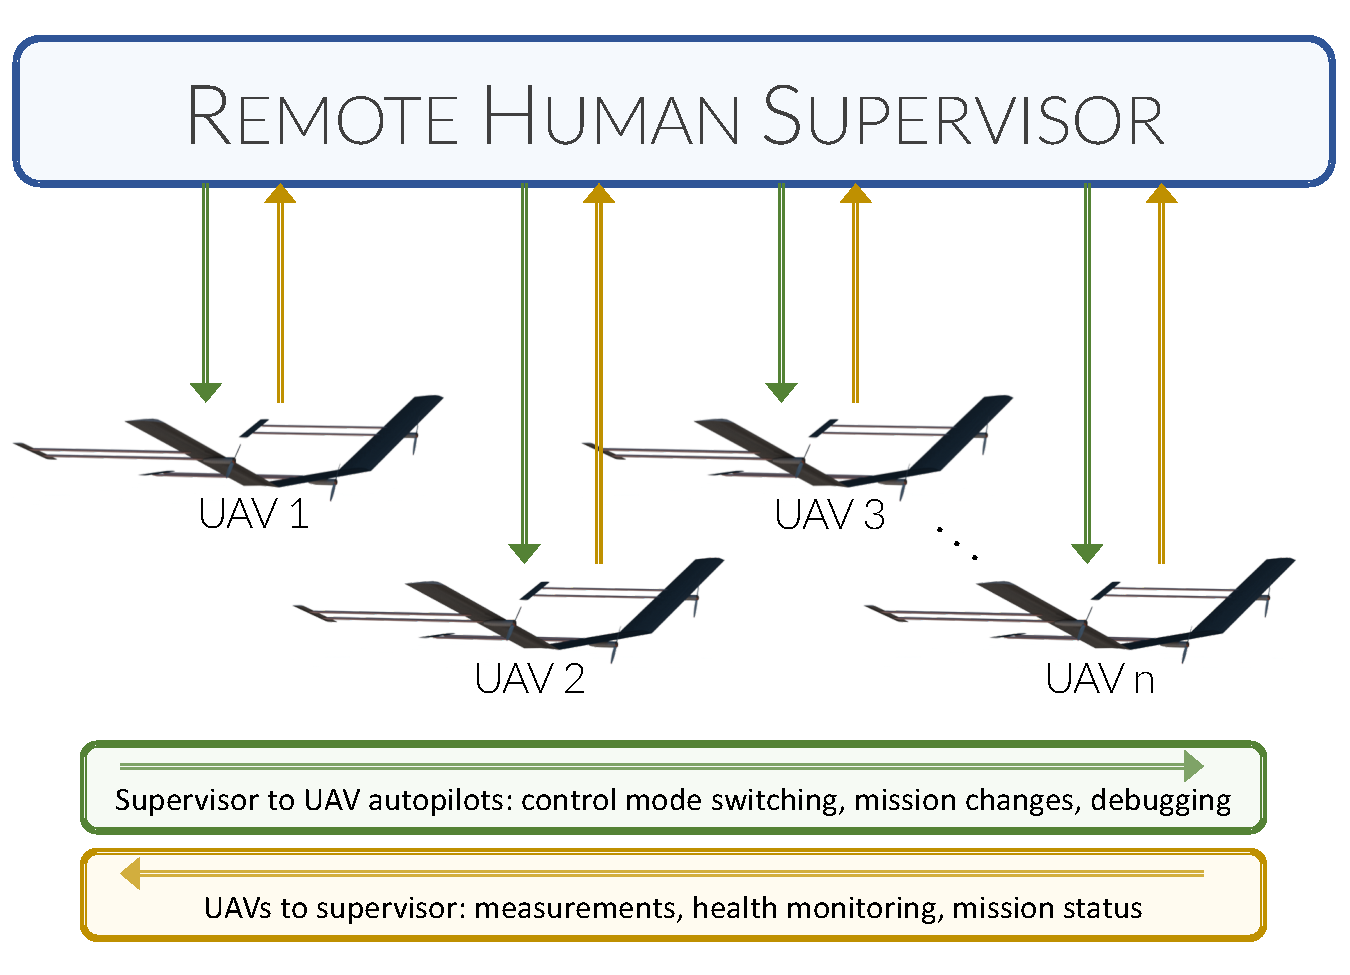
\includegraphics[width=0.95\columnwidth]{../fig/uav_supervisor.pdf}
	\caption{Supervisory remote operation of HALE UAVs}
	\label{fig:uav_supervisor}
\end{figure}

%\textit{Human-in-the-loop} operation is possible via remote controls, allowing the operator to actuate the plant by manually providing $u(t)$ in (\ref{eq:first_order_act}) and (\ref{eq:second_order_act}). Manual remote control introduces communication time delays $(\tau_y, \tau_u) > 0$, in sensing and actuation, respectively.

%Recovery of closed-loop autonomous control performance following the introduction of severe anomalous dynamics to the plant. 

%Human supervisor is present (remotely), but should not be given control responsibilities following anomaly.

\section{Shared Controller}\label{sec:shared_ctrl}
%Overview of shared control architecture. What is assumed?
%We introduce a shared decision-making and control framework with the goal of enabling the safe operation of HALE UAVs subject to both parametric uncertainties and the sudden introduction of anomalous, unmodeled dynamics as described in the preceding section. The shared control framework is based on a combination of actions by UAV autopilots and remote human operators. MRAC autopilots and complementary higher-level motion planning algorithms allow for continuous autonomous operation of the UAVs under nominal conditions. Remote human operators monitor the performance of the vehicles and are trained and able to remotely pilot the vehicle in case of autopilot failure. The remote piloting of the vehicles, however, is a daunting task due to communication delays and a weakened understanding of the vehicle dynamics, state, and environment, due to the remote nature of the task. Our shared anomaly response involves the remote human operator to diagnose and correct for the dynamical anomaly without taking over manual control of the vehicle. In Section \ref{subsec:sc_adaptive}, we describe two adaptive autopilot designs, which, in combination with the human operator whose precise role is described subsequently in Section \ref{subsec:sc_human}, will solve the problem presented in Section \ref{sec:problem}.
We introduce a shared decision-making and control framework in a flight platform subject to both parametric uncertainties and the sudden introduction of anomalous, unmodeled dynamics as described in the preceding section. The shared control framework is based on a combination of actions by autonomous control algorithms and remote human operators. MRAC autopilots allow for continuous autonomous operation of the vehicle under nominal conditions. Remote human operators monitor the performance of the vehicles and are trained and able to remotely pilot the vehicle in case of autopilot failure. %
%The remote piloting of the vehicles, however, is a daunting task due to communication delays and a weakened understanding of the vehicle dynamics, state, and environment, due to the remote naturs of the task. 
Our shared anomaly response involves the remote human operator to diagnose and correct for the dynamical anomaly without taking over manual control of the vehicle. In Section \ref{subsec:sc_adaptive}, we describe two adaptive autopilot designs, which, in combination with the human operator whose precise role is described subsequently in Section \ref{subsec:sc_human}, will solve the problem presented in Section \ref{sec:problem}.

%Division of responsibilities.

\subsection{Adaptive Output-Feedback Control}\label{subsec:sc_adaptive}
An autonomous controller is designed to track prescribed commands for plant outputs $z_p(t)$ in (\ref{eq:plant_dynamics}), and is described in detail in this section. % The shared control framework involves separate MRAC designs for the plant (\ref{eq:plant_dynamics}) in combination with actuator dynamics (\ref{eq:first_order_act}) and (\ref{eq:second_order_act}). The control design accommodating first-order actuators is denoted the ``nominal'' control design, and excluding exceptional failures, is the controller in use by the UAV autopilot. The control design accommodating second-order actuators is a predefined ``recovery'' controller, whose use case will be defined more fully in Section \ref{subsec:sc_human}. 
To achieve the control goals stated in Section \ref{sec:problem}, our proposed autopilot includes two components:
\begin{enumerate}[label=(\roman*)]
	\item baseline control design using the robust servomechanism linear quadratic regulator method (RSLQR);
	\item adaptive output-feedback augmentation for parametric uncertainties in the plant.
\end{enumerate}

%Control design in each case uses an augmented linear plant formulation, where the plant (\ref{eq:plant_dynamics}) is extended with the actuator dynamics -- either (\ref{eq:first_order_act}) or (\ref{eq:second_order_act}) -- as well as integrated tracking errors 
An additional integral error state is included as
\begin{equation}
	e_z^{\mathcal{I}}(t) = \int_0^{t} \big( z_p(\tau) - z_{cmd}(\tau)\big) d\tau.
\end{equation}

The augmented plant model with $x = \begin{bmatrix} x_p^T & x_{act}^T & (e_z^{\mathcal{I}})^T\end{bmatrix}^T$ can written compactly as
\begin{equation}
\begin{array}{c}
\dot{x}= \left(A+B_{1}\Psi_{1}^{T}+B_{r}\Psi_{r}^{T}\right) x+B_{r}\Lambda u+B_{z}z_{cmd}\\
y=Cx,\qquad z=C_{z}x
\end{array} \label{eq:augmented_plant}
\end{equation}
where $x\in\mathbb{R}^{n}$, $u\in\mathbb{R}^{m}$, $y\in\mathbb{R}^{p}$ are redefined states, inputs and outputs, respectively. 
%A full justification for this form of the plant can be found in \cite{qu2016phd, qu2016adaptive}. 
This plant contains unknown matrices $\Psi_1$, $\Psi_r$, and $\Lambda$, which hold the state-dependent plant uncertainties, state-dependent actuator dependencies, and actuator effectiveness, respectively. We consider square plants with $m = p$. The subscript $r$ indicates the relative degree of the augmented plant, and the definitions of $B_r$ and $\Psi_r$ depend on whether the actuators are first-order (\ref{eq:first_order_act}) or second-order (\ref{eq:second_order_act}). It is noted that the augmented plant model which arises from the inclusion of actuator model (\ref{eq:first_order_act}) in the plant (\ref{eq:plant_dynamics}) has relative degree two, while the augmented plant model associated with the inclusion of actuator model (\ref{eq:second_order_act}) has relative degree three. 

For control design, closed-loop reference models (\cite{gibson2013adaptive}) are designed as
\begin{equation}
\dot{x}_m = A_m x_m + B_z z_{cmd} + L e_y + \mathcal{F}_r(t), \quad y_m = C x_m
\end{equation}
where $e_y = y - y_m$, $A_m = A - B_r K^T$ with $K\in\mathbb{R}^{n\times m}$ is a baseline feedback control gain designed for the system without uncertainty using RSLQR, as described by \cite{lavretsky2013robust}. $L$ is a Luenberger-like residual feedback gain, and $\mathcal{F}_r(t)$ is a function used when $r \geq 2$ to recover stability properties in the presence of uncertainty. 

In what follows, we introduce a ``nominal'' adaptive autopilot design for plants of the form (\ref{eq:augmented_plant}) having relative degree two and parametric uncertainties $\Psi_1$, $\Psi_2$, and $\Lambda$. We then introduce a ``recovery'' adaptive autopilot design for plants of the form (\ref{eq:augmented_plant}) with relative degree three due to an anomaly, and uncertainties $\Psi_1$, $\Psi_3$, and $\Lambda$. Readers are referred to \cite{qu2016phd} and \cite{qu2016adaptive} for a thorough derivation of adaptive control design for plants having arbitrary relative degree. 
 
\subsubsection{Nominal Adaptive Control Design}
%Relative degree two MIMO adaptive control.
% need a11, a10, B_1^a, Cbar, S, Rinv, epsilon, L, two tuner laws, u, F
The control design for the plant with first-order actuator dynamics is summarized by providing definitions for CRM residual gain matrix $L$, function $\mathcal{F}_2(t)$, control law $u(t)$, and parameter adaptation. Note that $B_2$ represents $B_r$ from (\ref{eq:augmented_plant}) for this relative degree two plant. 

The feedback matrix $L$ is designed as follows. We define the ``relative degree one input path''
\begin{equation}
B_1^a = \alpha_0 B_2 + \alpha_1 A B_2 \label{eq:rd2-b1a}
\end{equation}
where $\alpha_i > 0$ are free design parameters. We then define
\begin{align}
S &= (C B_1^a)^T \label{eq:S}\\	\overline{C} & = S C\\ R^{-1} &= (\overline{C} B_1^a)^{-1} \big[ \overline{C} A B_1^a + (\overline{C} A B_1^a)^T\big] (\overline{C} B_1^a)^{-1} + \epsilon I \\ L & = B_1^a R^{-1} S \label{eq:L}
\end{align}
where $\epsilon > 0$ \cite[Eq. 30]{qu2015adaptive} is chosen to guarantee stability of the adaptive system. 

The function $\mathcal{F}_2(t)$ makes use of scaled error signal
\begin{equation}
	e_{sy}(t) = R^{-1} S e_y(t) \label{eq:esy}
\end{equation}
and a filtered version of this signal, $\overline{e}_{sy}(t)$, given in the form of a differential equation as
\begin{equation}
(\alpha_0 + \alpha_1 \frac{d}{dt}) \big\{ \overline{e}_{sy}(t) \big\} = \alpha_1 e_{sy}(t). \label{eq:e_sy_bar}
\end{equation}
It is worth noting that this can be represented in the Laplace $s$-domain with a first-order filter
\begin{equation*}
	\overline{E}_{sy}(s) = \frac{\alpha_1}{\alpha_1 s + \alpha_0} E_{sy}(s).
\end{equation*}

$\mathcal{F}_2(t)$ is then defined as
\begin{equation}
\mathcal{F}_2(t) = B_2 (\alpha_0 + \alpha_1 \frac{d}{dt})\big\{ \hat{\Psi}_m^T (t) \bar{e}_{sy}(t) \big\} \label{eq:F2}
\end{equation}
where $\hat{\Psi}_m(t)$ is a matrix of adaptive parameters. Similar to (\ref{eq:e_sy_bar}), we define filtered reference model state, $\overline{x}_m(t)$, with the differential equation
\begin{equation}
(\alpha_0 + \alpha_1 \frac{d}{dt}) \big\{ \overline{x}_{m}(t) \big\} = \alpha_1 x_{m}(t). \label{eq:xm_bar}
\end{equation}

We define a regressor vector of known signals as
\begin{equation}
\mathcal{X}(t) = \big[ (K^T \overline{x}_m)^T,\quad x_m^T,\quad \overline{x}_m^T \big]^T.
\end{equation}

The control law, $u(t)$, is then given by
\begin{equation}
u(t) = - (\alpha_0 + \alpha_1 \frac{d}{dt}) \big \{ \hat{\Psi}_{\Lambda}^T (t) \mathcal{X}(t) \big\} \label{eq:u_rd2}	
\end{equation}
where $\hat{\Psi}_{\Lambda}(t)$ is a matrix of adaptive parameters. The laws for adaptation of parameter matrices $\hat{\Psi}_m(t)$ and $\hat{\Psi}_{\Lambda}(t)$ are given by
\begin{equation}
\begin{aligned}
	\dot{\hat{\Psi}}_m(t) &= \Gamma_{m} \overline{e}_{sy}(t) e_y^T(t) S^T \\
	\dot{\hat{\Psi}}_{\Lambda}(t) &= -\Gamma_{\Lambda} \mathcal{X}(t) e_y^T (t) S^T
\end{aligned} \label{eq:rd2-adaptation}
\end{equation}
with diagonal adaptation gains $\Gamma_{m}, \;\Gamma_{\Lambda} > 0$. We note that the derivatives of the adaptive parameters, computed in (\ref{eq:rd2-adaptation}), are used to implement (\ref{eq:F2}) and (\ref{eq:u_rd2}) with the product rule of differentiation.

\subsubsection{Recovery Adaptive Control Design}
Control design with the second-order actuator model is similar to the nominal control design, but requires modifications to ensure strict positive realness of the transfer matrix of the model-following error dynamics. 

The definition of $L$ is modified by replacing $B_1^a$ in (\ref{eq:rd2-b1a}) with
\begin{equation}
B_1^a = \alpha_0 B_3 + \alpha_1 A B_3 + \alpha_2 A^2 B_3 \label{eq:rd3-b1a}
\end{equation}
and proceeding with (\ref{eq:S})--(\ref{eq:L}). A definition for $\epsilon>0$ in this case can be found in \cite{qu2016phd}. To simplify notation, the operator $\Pi \{\cdot \}$ is defined as
\begin{equation}
\Pi \{ \cdot \} = \big( \alpha_0 + \alpha_1 \frac{d}{dt} + \alpha_2 \frac{d^2}{dt^2} \big) \{ \cdot \}.
\end{equation}

The function $\mathcal{F}_3(t)$ utilizes filtered error vectors $\overline{e}_{sy}^{[1]}(t)$, $\overline{e}_{sy}^{[2]}(t)$, and $\overline{e}_{sy}^{[1][2]}(t)$, defined by the differential equations
\begin{equation}
\begin{aligned} 
	\Pi \big \{ \overline{e}_{sy}^{[1]}(t) \big \} & = (\alpha_1 + \alpha_2 \frac{d}{dt}) \big \{ e_{sy}(t) \big \} \\
	\Pi \big \{ \overline{e}_{sy}^{[2]}(t) \big \} & = \alpha_2 e_{sy}(t) \\
	\Pi \big \{ \overline{e}_{sy}^{[1][2]}(t) \big \} & = (\alpha_2 \frac{d}{dt}) \big \{ \hat{\phi}_1^T(t) \bar{e}_{sy}^{[1]}(t) \big \}
\end{aligned} \label{eq:esy_rd3}
\end{equation}
where $e_{sy}(t)$ was defined in (\ref{eq:esy}), $\hat{\phi}_1(t)$ is a vector of adaptive parameters, and coefficients $\alpha_i > 0$ are free design parameters. We define the integrated and scaled measurement output error, 
\begin{equation}
e_{y}^{\mathcal{I}}(t) = \int_0^{t} L\big (y(\tau) - y_m(\tau)\big) d\tau
\end{equation}
which is used to define filtered error signals $\overline{e}_{\mathcal{I}y}^{[1]} (t)$ and $\overline{e}_{\mathcal{I}y}^{[1][2]} (t)$, given by
\begin{equation}
\begin{aligned}
	\Pi \big \{  \overline{e}_{\mathcal{I}y}^{[1]} (t) \big \} &= (\alpha_1 \frac{d}{dt} + \alpha_2 \frac{d^2}{dt^2}) \big \{ \hat{\Phi}_1^T (t) e_{y}^{\mathcal{I}}(t) \big \} \\
	\Pi \big \{  \overline{e}_{\mathcal{I}y}^{[1][2]} (t) \big \} &= (\alpha_2 \frac{d}{dt}) \big \{ \hat{\Lambda}(t) \overline{e}_{\mathcal{I}y}^{[1]} (t) \big \}
\end{aligned} \label{eq:eIy_rd3}
\end{equation}
where $\hat{\Phi}_1(t)$ and $\hat{\Lambda}(t)$ are matrices of adaptive parameters. We define operators
\begin{equation}
\begin{aligned}
	f_a \{ \cdot \} &= \big(\alpha_0 \alpha_2 B_3 + (\alpha_1 B_3 + \alpha_2 A B_3)\frac{d}{dt} \big) \{ \cdot \} \\
	f_b \{ \cdot \} &= \alpha_2 B_3 \Pi \{ \cdot \}
\end{aligned}
\end{equation}
and use these to define
\begin{multline}
	\mathcal{F}_3(t) = f_a \big \{ \hat{\phi}_1^T(t) \overline{e}_{sy}^{[1]}(t) - \hat{\Lambda}^T(t) \overline{e}_{\mathcal{I}y}^{[1]} (t) \big \} \\
	+ f_b \big \{ \hat{\phi}_1^T(t) \big[\overline{e}_{sy}^{[1][2]}(t) -  \overline{e}_{\mathcal{I}y}^{[1][2]} (t) \big ] + \hat{\phi}_2^T (t) \overline{e}_{sy}^{[2]}(t) \big \} \label{eq:F3}
\end{multline}
where $\hat{\phi}_2(t)$ is an additional vector of adaptive parameters. 

We define filtered reference model states $\overline{x}_m^{[1]}$ and $\overline{x}_m^{[2]}$ as
\begin{equation}
\begin{aligned}
	\Pi \big \{  \overline{x}_{m}^{[1]} (t) \big \} &= (\alpha_1 + \alpha_2 \frac{d}{dt}) \big \{ x_m (t) \big \} \\
	\Pi \big \{  \overline{x}_{m}^{[2]}(t) \big \} &= \alpha_2 x_m (t).
\end{aligned}	
\end{equation}

Variable $\overline{v}_m(t)$ is introduced, with artificial time derivatives, such that
\begin{equation}
\begin{gathered}
	\overline{v}_m = x_m, \quad \frac{d }{dt}\{ \overline{v}_m \} = A x_m + B_z z_{cmd} \\
	\frac{d^2}{dt^2} \{ \overline{v}_m \} = A^2 x_m + A B_z z_{cmd} + B_z \frac{dz_{cmd}}{dt} - A L e_y.
\end{gathered}
\end{equation}

The regressor vector $\mathcal{X}(t)$ is redefined as
\begin{equation}
\mathcal{X}(t) = \big[ (K^T \overline{x}_m^{[2]})^T,\quad \overline{v}_m^T,\quad \overline{x}_m^{[1]T},\quad \overline{x}_m^{[2]T} \big]^T.
\end{equation}

The control law $u(t)$ for the ``recovery'' controller is
\begin{equation}
\begin{aligned}
	u (t) = -&\Pi \big \{ \hat{\Psi}^T(t) \mathcal{X}(t) \big \} \\ - & (\alpha_1 \frac{d}{dt} + \alpha_2 \frac{d^2}{dt^2}) \big \{ \hat{\Phi}_1^T(t) \big \} e_y^\mathcal{I} (t) 
\end{aligned} \label{eq:u_rd3}
\end{equation}
where 
\begin{equation}
\hat{\Psi}(t) = \big[ \hat{\Upsilon}^T(t),\quad \hat{\Phi}_1^T(t),\quad \hat{\Phi}_2^T(t),\quad \hat{\Phi}_3^T(t) \big]^T 
\end{equation}
is a matrix of adaptive parameters. 

In this controller, the adaptive parameters are adjusted using second-order tuners as in \cite{qu2016phd}. We first define a regressor vector $\nu(t)$ of filtered error signals
\begin{equation}
	\nu(t) = \begin{bmatrix}
		(\overline{e}_{\mathcal{I}y}^{[1][2]} - \overline{e}_{sy}^{[1]} - \overline{e}_{sy}^{[1][2]})^T, & \quad (-\overline{e}_{sy}^{[2]})^T, & \quad (\overline{e}_{\mathcal{I}y}^{[1]})^T
	\end{bmatrix}^T
\end{equation}
and associated matrix of adaptive parameters
\begin{equation}
\hat{\Theta}(t) = \big[ \hat{\phi}_1^T(t),\quad \hat{\phi}_2^T(t),\quad \hat{\Lambda}^T(t) \big].
\end{equation}

Inputs to the second-order tuners are calculated by integrating
\begin{equation}
\begin{aligned}
\dot{\hat{\Psi}}'(t) &= \Gamma_{\Psi} \mathcal{X} e_y^T S^T \text{sgn}(\Lambda) \\
\dot{\hat{\Theta}}'(t) &= -\Gamma_{\Theta} \nu e_y^T S^T
\end{aligned}
\end{equation}
where $\Gamma_{\Psi}, \Gamma_{\Theta} > 0$ are diagonal adaptation gains. 

The desired matrices of adaptive parameters are outputs of the tuners
\begin{equation}
\begin{aligned}
	\dot{X}_{\hat{\Psi}}(t) &= \big( A_T X_{\hat{\Psi}} + B_T (\hat{\Psi}'(t))^T \big) g(\mathcal{X}, \mu_{\mathcal{X}}) \\
	\hat{\Psi}(t) &= (C_T X_{\hat{\Psi}})^T \\
	\dot{X}_{\hat{\Theta}}(t) &= \big( A_T X_{\hat{\Theta}} + B_T (\hat{\Theta}'(t))^T \big) g(\nu, \mu_{\nu}) \\
	\hat{\Theta}(t) &= (C_T X_{\hat{\Theta}})^T
\end{aligned}	
\end{equation}
where
\begin{equation}
g(\mathbf{x}, \mu) = 1 + \mu \mathbf{x}^T \mathbf{x}	
\end{equation}
is a time-varying gain with scalar gain $\mu$ described in \cite{qu2016phd}. $A_T \in \mathbb{R}^{2m \times 2m}$, $B_T \in \mathbb{R}^{2m \times m}$, and $C_T \in \mathbb{R}^{m \times 2m}$ are block diagonal matrices with diagonal blocks
\begin{equation}
A_{T,i} = \begin{bmatrix}
	0 & 1\\ -\frac{\alpha_0}{\alpha_2} & -\frac{\alpha_1}{\alpha_2}
\end{bmatrix}, \quad B_{T,i} = \begin{bmatrix}
	0 \\ \frac{\alpha_0}{\alpha_2}
\end{bmatrix}, \quad C_{T,i} = \begin{bmatrix}
	1 & 0
\end{bmatrix}
\end{equation}

Derivatives of the adaptive parameters, used in (\ref{eq:esy_rd3}), (\ref{eq:eIy_rd3}), (\ref{eq:F3}), and (\ref{eq:u_rd3}), are given by
\begin{equation}
\begin{aligned}
	\dot{\hat{\Psi}}(t) &= (C_T^\delta X_{\hat{\Psi}})^T, \qquad \ddot{\hat{\Psi}}(t) &= (C_T^{\delta\delta}X_{\hat{\Psi}})^T \\
	\dot{\hat{\Theta}}(t) &= (C_T^\delta X_{\hat{\Theta}})^T, \qquad \ddot{\hat{\Theta}}(t) &= (C_T^{\delta\delta}X_{\hat{\Theta}})^T
\end{aligned} \label{eq:rd3-adaptation-deriv}
\end{equation}
where $C_T^{\delta}, C_T^{\delta \delta} \in \mathbb{R}^{m \times 2m}$ are block diagonal matrices with diagonals $C_{T,i}^{\delta} = \begin{bmatrix} 0,~ & 1	\end{bmatrix}$ and $C_{T,i}^{\delta\delta} = -\frac{1}{\alpha_2}\begin{bmatrix} \alpha_0,~ & \alpha_1 \end{bmatrix}$. 

\subsection{Human Supervisor}\label{subsec:sc_human}
%Notices, reacts, instructs.
We task the remote human supervisor with the following three responsibilities for shared anomaly response.
\begin{enumerate}[label=Task \arabic*., leftmargin=1.4cm]
	\item Timely detection and characterization of anomalous closed-loop dynamical behavior
	\item Isolation of control loop with anomalous behavior (i.e. longitudinal or lateral-directional)
	\item Commanding a change from nominal autopilot (\ref{eq:rd2-b1a})--(\ref{eq:rd2-adaptation}) to recovery autopilot (\ref{eq:rd3-b1a})--(\ref{eq:rd3-adaptation-deriv})
\end{enumerate}

The first task requires an attentive human operator able to discern that 
\begin{enumerate}[label=(\alph*)]
	\item an anomaly has occurred and control performance degradation is not caused solely by external disturbances;
	\item swift action must be taken in order to recover stability and performance;
	\item it may be possible to recover stability and performance via corrective action.
\end{enumerate}

The second task requires a human operator with knowledge and familiarity with the plant dynamics and control structure to understand which control loop (e.g. pitch mode, roll mode, airspeed, in a fixed-wing UAV application) is the source of the anomalous dynamics. 

The final task for the trained remote human operator is the transfer of this diagnosis to the autopilot, by changing the relevant controller to its ``recovery'' mode.

\subsection{Overall Shared Control Architecture}\label{subsec:sc_overall}

The shared control architecture between adaptive autopilots and a human operator that we propose is as follows. Before the occurrence of an anomaly, the nominal adaptive autopilot with control action defined in (\ref{eq:u_rd2}) is used to control the plant. An anomaly which suddenly changes actuator dynamics from (\ref{eq:first_order_act}) to (\ref{eq:second_order_act}) is assumed to occur at $t := t_1^*$. Following this time instant, the human operator is responsible for carrying out tasks 1--3 before the time limit at which failure would occur without action ($t:=t_3^*$). The completion of task 3 by the human ($t := t_2^*$) results in a switch to the recovery adaptive autopilot with control action as in (\ref{eq:u_rd3}). 

Note that our shared control architecture does not involve a handover of regulation and command tracking tasks to the human following an anomaly. We hypothesize that such a division of authority, in which the human operator is responsible for high-level cognition tasks while adaptive autopilots retain responsibility for low-level regulation, results in a shared control architecture which leverages the capabilities of these two decision-makers.

A detailed discussion of the stability of the resulting controller is not carried out in this paper. But it is clear that if the human completes tasks 1--3 sufficiently fast ($t_2^* < t_3^*$), the adaptive controller will guarantee boundedness of the closed-loop system and convergence of $e(t) = x(t) - x_m(t)$ to zero if our assumptions are satisfied. We carry out a detailed simulation study in the following section and evaluate the performance of the shared controller proposed above.

\section{Anomaly Response Simulations} \label{sec:vfa}
%HALE VFA.
The shared control solution introduced in Section \ref{sec:shared_ctrl} is applied to the problem introduced in Section \ref{sec:problem} on a high altitude, long endurance (HALE) model. HALE aerial platforms, such as the solar-electric NASA/AeroVironment Helios and Facebook Aquila, have unique design considerations to satisfy goals of uninterrupted weeks- or months-long operation. To reduce power draw, HALE aircraft designs save mass by allowing wings to bend, and may be classified as very flexible aircraft (VFA). Compared to typical fixed-wing aircraft, these aircraft operate at low speed, and may use low-bandwidth actuators which must be accounted for in control design. HALE VFA platforms are likely to have significant modeling uncertainties and online variation in dynamics due to flexible effects and degradation over long-term operation. Although these vehicles are unmanned, they require supervision from remote human operators.

The aircraft model used in simulation, developed by \cite{gibson2011modeling} for longitudinal control design applications, is rendered in Figure \ref{fig:vfa} and described in Section \ref{subsec:vfa_model}. The results of numerical simulations on the control and anomaly recovery with this MIMO plant are then presented in Section \ref{subsec:sims}, comparing the shared anomaly response to alternative anomaly responses.

\subsection{Aircraft Model}\label{subsec:vfa_model}
\begin{figure}[htbp]
	\centering
	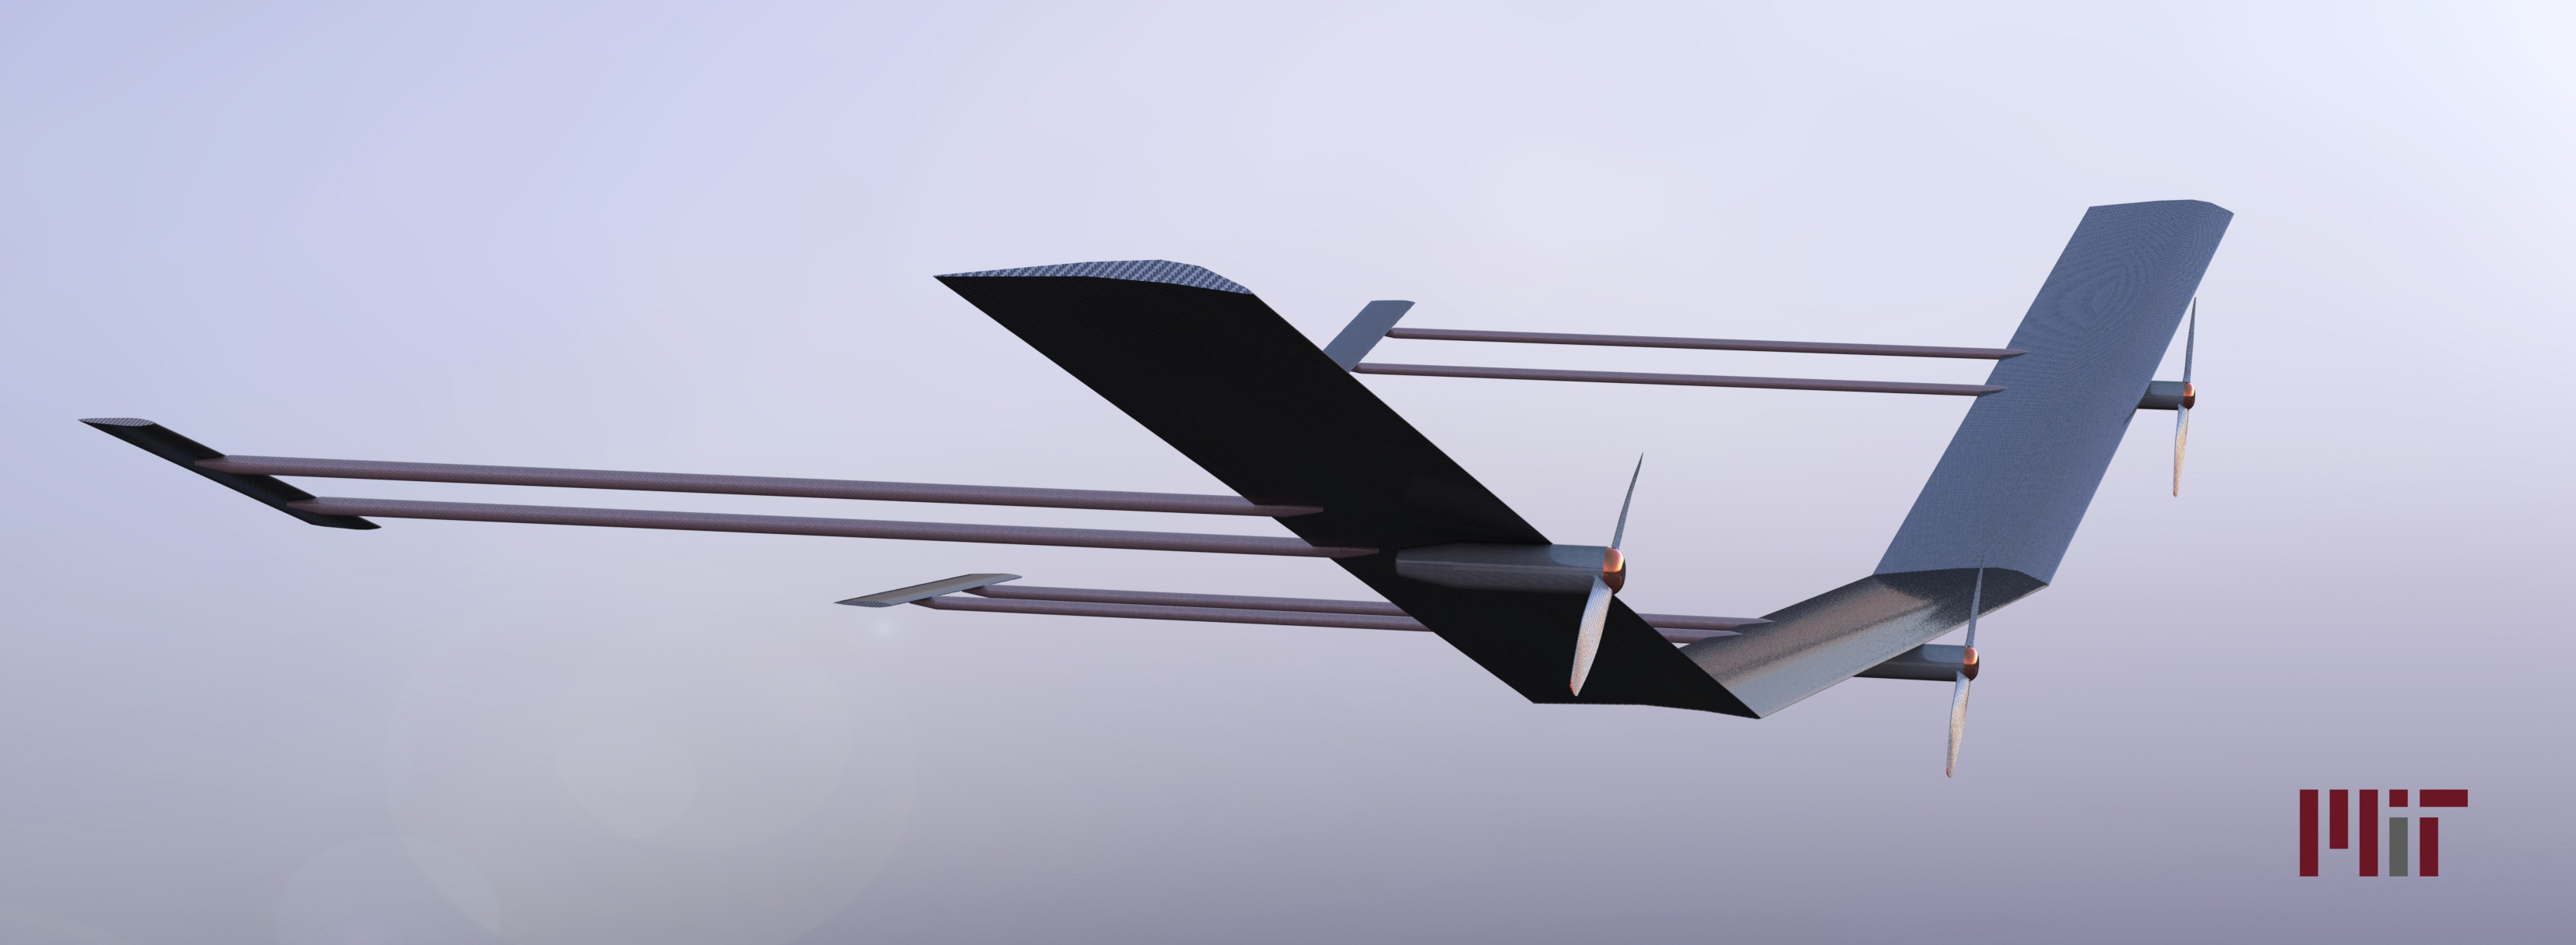
\includegraphics[width=0.95\columnwidth]{../fig/VFA_16.jpg}
	\caption{Rendering of very flexible aircraft model}
	\label{fig:vfa}
\end{figure}

The aircraft model used in simulation represents the nonlinear longitudinal dynamics of a HALE VFA concept with three rigid lifting sections, hinged together such that the aircraft is able to bend at the joints of the three sections. The pitch mode dynamics of this nonlinear model is defined by the state vector
\begin{equation}
x_{\text{vfa}} = \begin{bmatrix}
~V~\\
\alpha \\
h \\
\theta \\
q\\
\eta\\
\dot{\eta}
\end{bmatrix} =
\begin{bmatrix}
	 $Airspeed (ft/s)$\\ $Angle of attack (rad)$\\ $Altitude (ft)$\\ $Pitch angle (rad)$\\ $Pitch rate (rad/s)$\\ $Dihedral (rad)$\\ $Dihedral rate (rad/s)$
\end{bmatrix}
\end{equation}

We linearize and trim the aircraft in straight and level flight using the inputs
\begin{equation}
	u_{\text{vfa}} = \begin{bmatrix}
\delta_{th} \\
\delta_{a,c} \\
\delta_{a,o} \\
\delta_{e,c} \\
\delta_{e,o} 
\end{bmatrix} = \begin{bmatrix}
		$Thrust (lbf)$\\
		$Center aileron (rad)$\\
		$Outer aileron (rad)$\\
		$Center elevator (rad)$\\
		$Outer elevator (rad)$
	\end{bmatrix}
\end{equation}

Assuming small deviations in altitude, the state vector corresponding to (\ref{eq:plant_dynamics}) is
\begin{equation}
	x_p = \begin{bmatrix}
V & \; \alpha & \; \theta & \; q & \; \eta & \; \dot{\eta}
\end{bmatrix}^T.
\end{equation}

We consider the control task of tracking commands for the dihedral angle and vertical acceleration, using control inputs $\delta_{a,o}$ and $\delta_{e,c}$ only, so the vector $u_p$ in (\ref{eq:plant_dynamics}) is
\begin{equation}
	u_p = \begin{bmatrix}
\delta_{a,o} & \; \delta_{e,c}
\end{bmatrix}^T.
\end{equation}

Regulation of the dihedral angle is desired, as a large dihedral angle is inefficient for lift generation and introduces instability in the open-loop dynamics, while a small dihedral angle will require more control effort to hold, increasing drag and power requirements and imparting twisting moments on the aircraft. 

The measurements available for control design are the pitch rate, dihedral angle, and vertical acceleration, leading to plant outputs
\begin{equation}
\begin{aligned}
y_p =& \, \Big[\; q \; \Big] \;= \Big[\: \text{Pitch rate (rad/s)} \:\Big] \\
z_p =& \begin{bmatrix}
\eta \\
A_z
\end{bmatrix} =\begin{bmatrix}
	$Dihedral angle (rad)$\\
	$Vertical acceleration (ft/s)$
\end{bmatrix}		
\end{aligned}
\end{equation}
and the outputs for the augmented plant (\ref{eq:augmented_plant}),
\begin{equation}
y = \begin{bmatrix}
	q \\ \int{z_p - z_{cmd}}
\end{bmatrix}, \quad z = z_p.
\end{equation}

For numerical simulations, the VFA model is trimmed at an airspeed of $68$ ft/s, altitude of $40,000$ ft, $2.8^\circ$ angle of attack and pitch angle (level flight), and dihedral angles ranging from $0$ to $20^\circ$ in $1^\circ$ increments. Figure \ref{fig:trim-poles} shows pole locations of the linearized plant for different dihedral angles, and Figure \ref{fig:trim-poles-zoom} shows instability of the linearized plant when trimmed above $11^\circ$ dihedral. Figure \ref{fig:trim-inputs} shows the thrust and control surface deflections for the trimmed VFA model over a range of dihedral angles.

\begin{figure}[htbp]
	\centering
	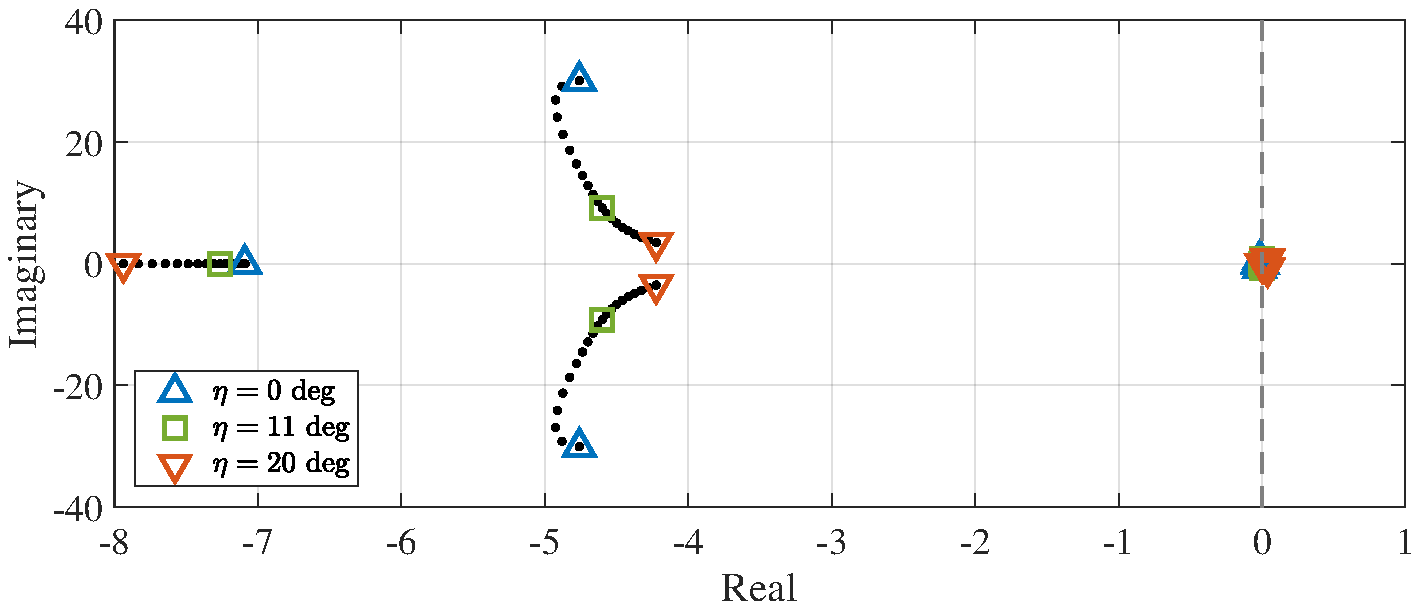
\includegraphics[width=0.95\columnwidth]{../fig/trim-poles-2.pdf}
	\caption{Poles of linearized system for different dihedral angles}
	\label{fig:trim-poles}
\end{figure}

\begin{figure}[htbp]
	\centering
	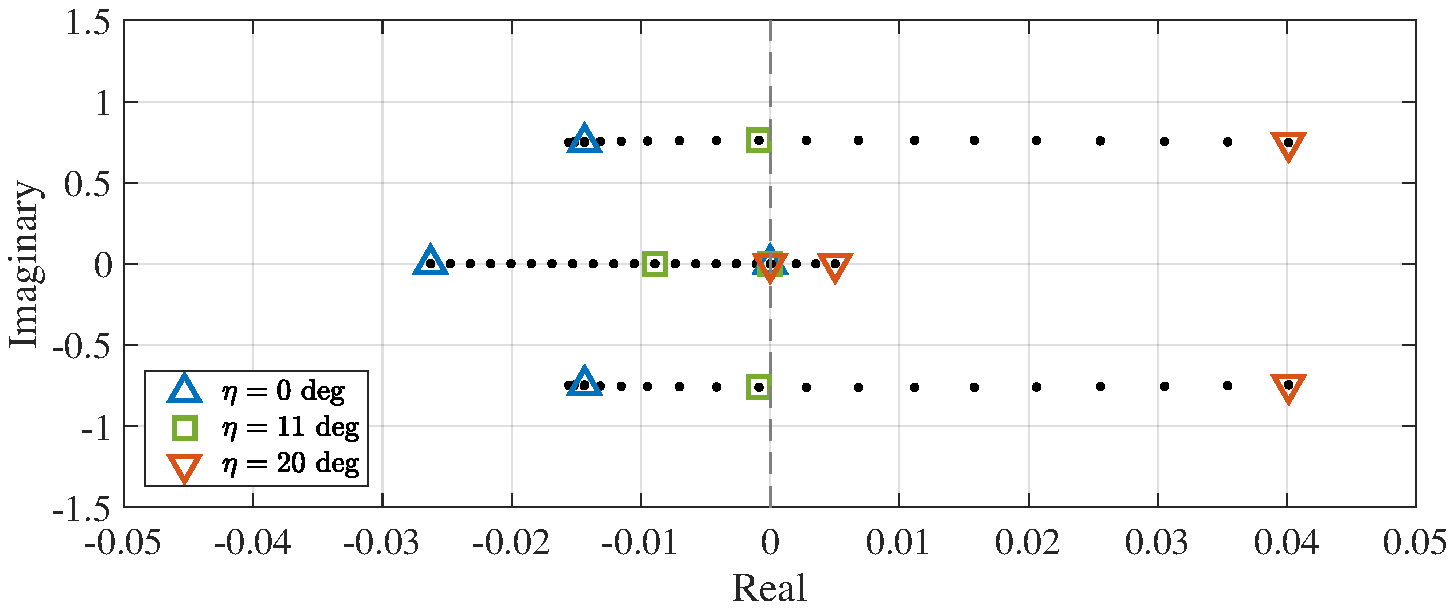
\includegraphics[width=0.95\columnwidth]{../fig/trim-poles-zoom-2.pdf}
	\caption{Dominant poles of linearized system, which move into the right-half complex plane when $\eta > 11^\circ$}
	\label{fig:trim-poles-zoom}
\end{figure}

\begin{figure}[htbp]
	\centering
	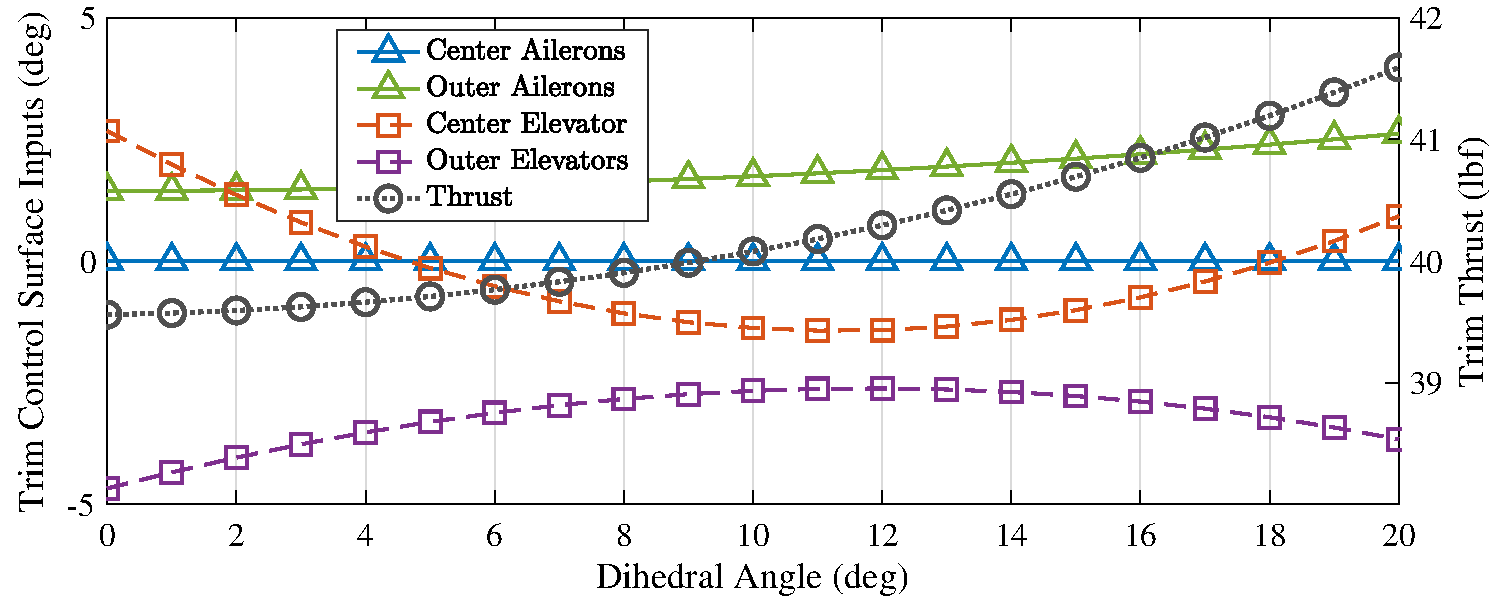
\includegraphics[width=0.95\columnwidth]{../fig/trim-inputs-3.pdf}
	\caption{Actuator trim at different dihedral angles}
	\label{fig:trim-inputs}
\end{figure}

The plant is augmented with a linear actuator model corresponding to (\ref{eq:first_order_act}) in the nominal case and (\ref{eq:second_order_act}) in the presence of anomalous dynamics. The vehicle simulation with first-order actuators (\ref{eq:first_order_act}) uses time constants $(\hat{\tau},\;\tau) = (0.5,\,2)$s in the control model and the actual plant, respectively, corresponding to
\begin{equation}
D_1 = 2 I_2, \quad \Theta_1 = -1.5 I_2
\end{equation}
where $\Theta_1$ is unknown for control design, and $I_2$ is the $2 \times 2$ identity matrix. 

Simulation of the anomalous dynamics (\ref{eq:second_order_act}) uses second-order actuators with cutoff frequencies $(\hat{\omega}_c,\; \omega_c) = (2 ,\; 1)$ rad/s and damping ratios $(\hat{\zeta},\; \zeta) = (0.7,\; 0.8)$ in the control model and actual plant, respectively, corresponding to
\begin{equation}
\begin{bmatrix}
	D_1 \\ D_2
\end{bmatrix} = \begin{bmatrix}
	4 I_2 \\ 2.8 I_2
\end{bmatrix}, \quad \begin{bmatrix}
	\Theta_1 \\ \Theta_2 
\end{bmatrix} = \begin{bmatrix}
	-3.75 I_2 \\ -2 I_2
\end{bmatrix}
\end{equation}
where $\Theta_1$ and $\Theta_2$ are unknown for control design. The uncertainty matrices $\Theta_p$ and $\Lambda$ are given by
\begin{equation}
\begin{gathered}
\Theta_{p}^{T}=\begin{bmatrix}
0.6 & -4.52 & \; 0 & \hfill 0.05 & \hfill 0.41 & \hfill 1.47\\
0.1 & \hfill 1.83 & \; 0 & -0.02 & -0.35 & -0.59
\end{bmatrix}\\ \Lambda = 0.2 I_2 \end{gathered}
\end{equation}
representing a poor linearization of the nonlinear model, and an 80\% reduction in actuator effectiveness.

\subsection{Numerical Simulations and Results} \label{subsec:sims}
We begin by simulating the HALE VFA under nominal autonomous control, responding to step inputs in commands for the dihedral angle and vertical acceleration, with the following three variants.
\begin{description}
	\item[Nom-1] Baseline RSLQR without uncertainty in control model
	\item[Nom-2] Baseline RSLQR with uncertainty in control model ($\Theta_p$, $\Lambda_p$, and $\Theta_1$)
	\item[Nom-3] Baseline RSLQR + MRAC with uncertainty in control model ($\Theta_p$, $\Lambda_p$, and $\Theta_1$)
\end{description}

\begin{figure}[htbp]
	\centering
	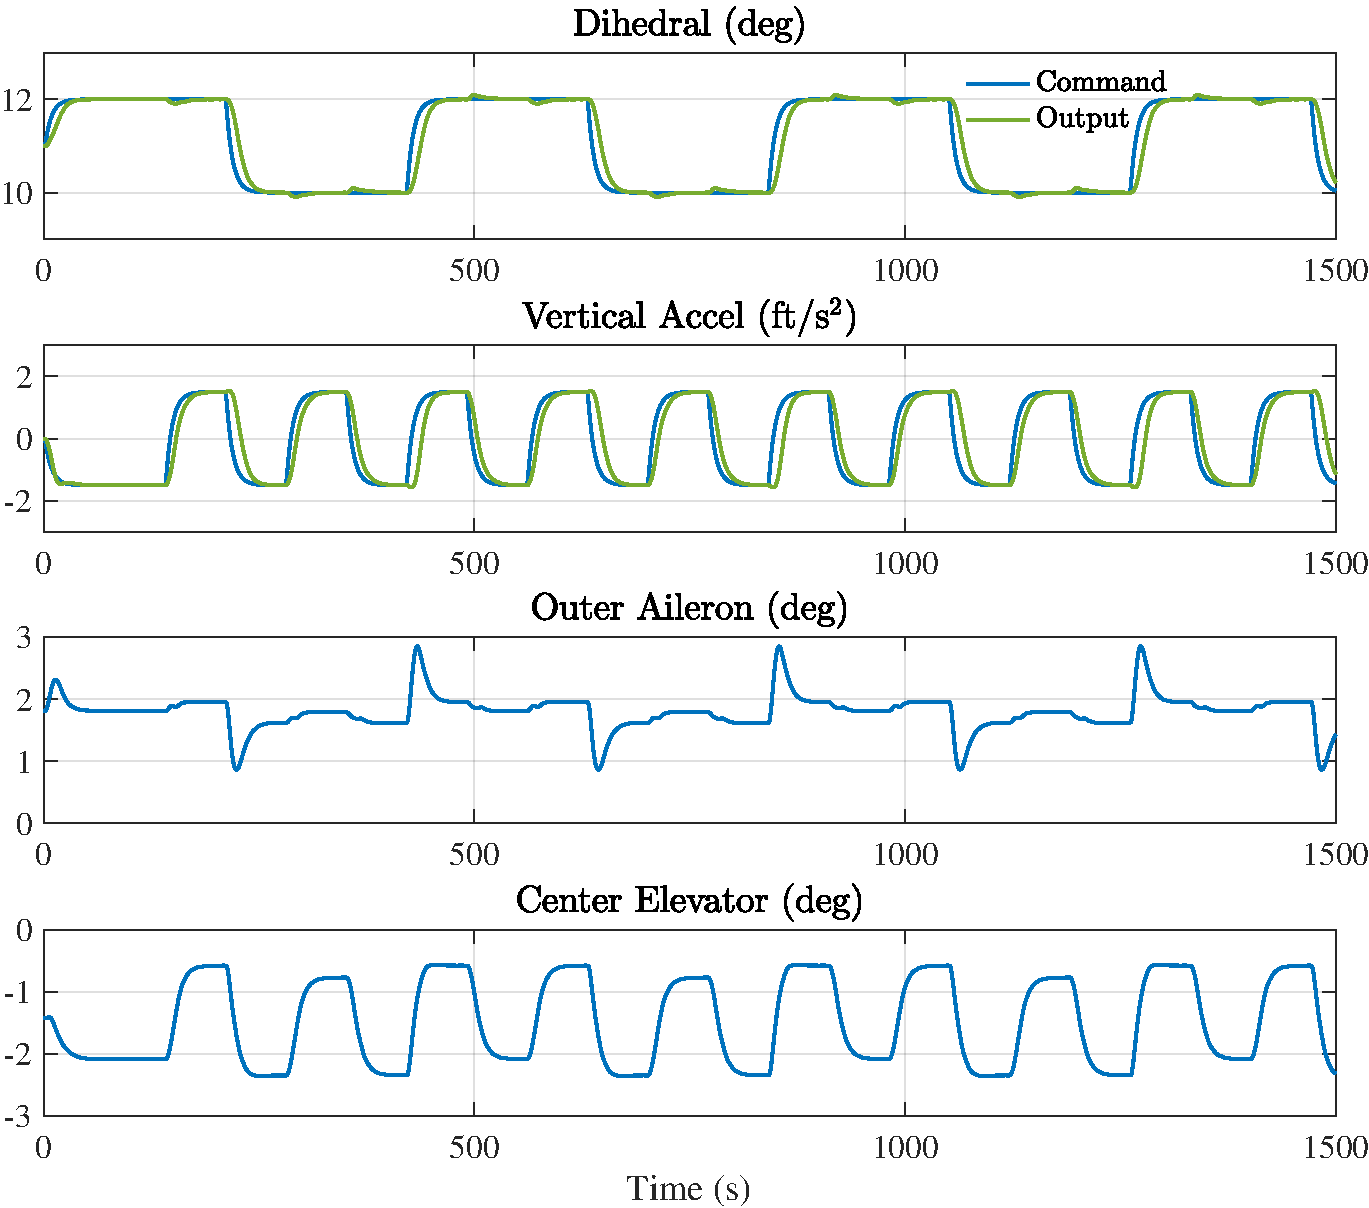
\includegraphics[width=\columnwidth]{../fig/nom1.pdf}
	\caption{Nom-1 simulation: RSLQR with no uncertainty in the control model}
	\label{fig:nom1}
\end{figure}

\begin{figure}[htbp]
	\centering
	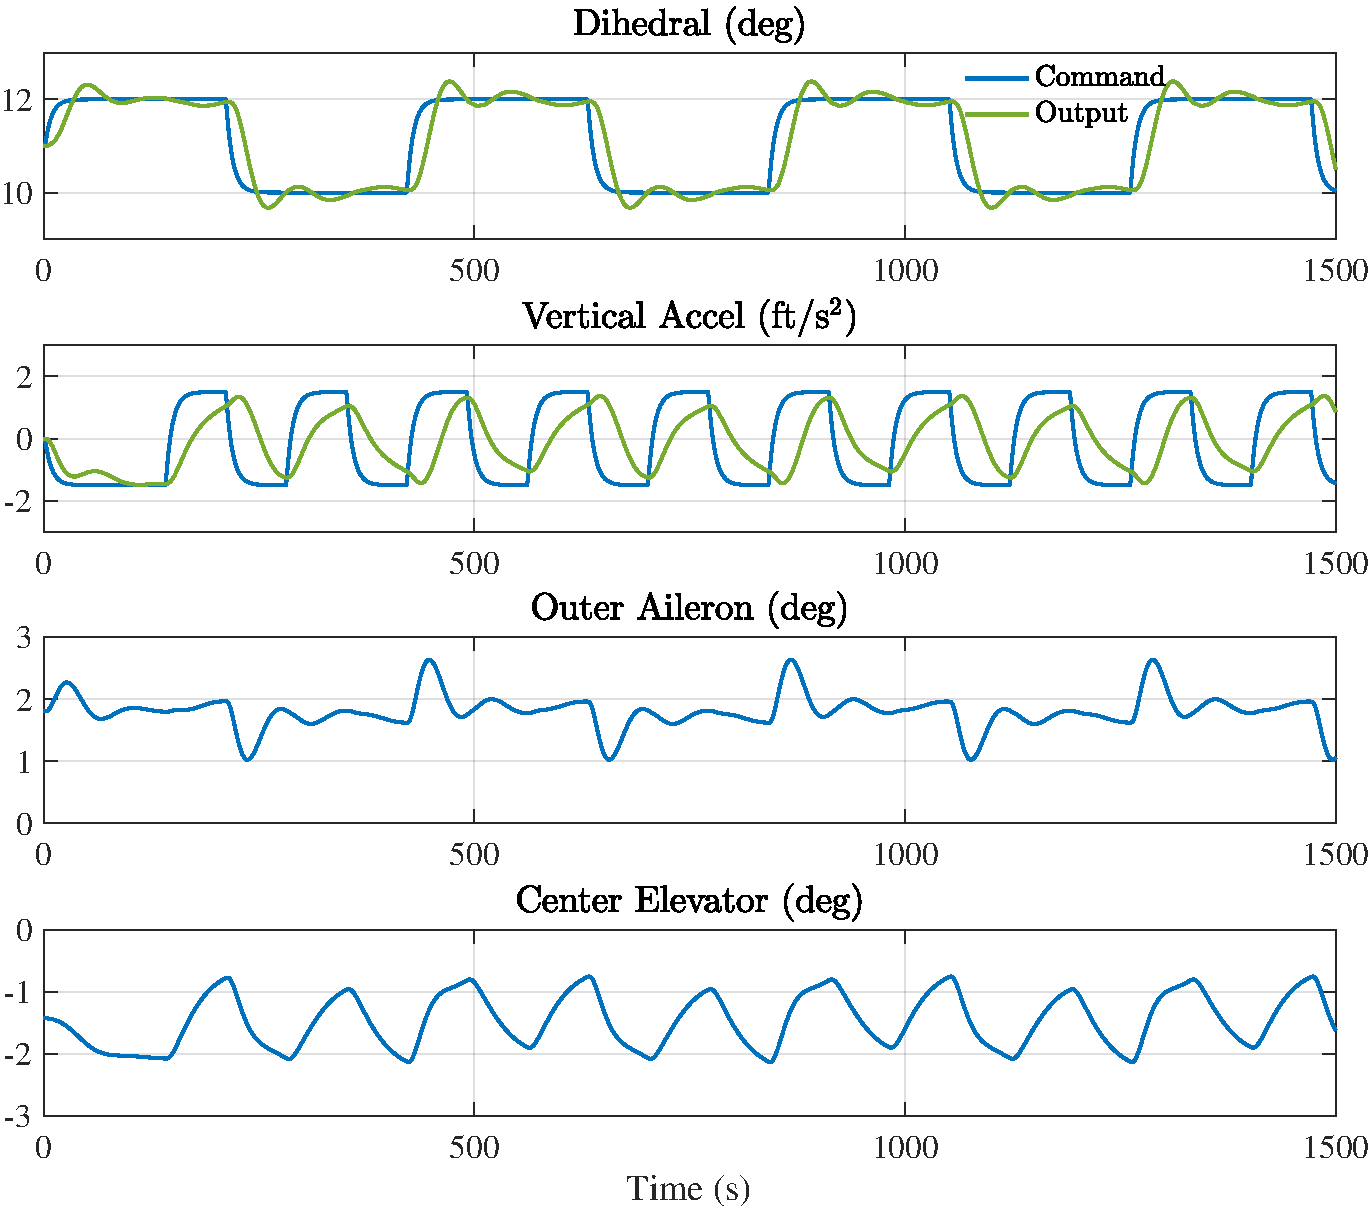
\includegraphics[width=\columnwidth]{../fig/nom2.pdf}
	\caption{Nom-2 simulation: RSLQR with uncertainties $\Theta_p$, $\Lambda_p$, and $\Theta_1$}
	\label{fig:nom2}
\end{figure}

\begin{figure}[htbp]
	\centering
	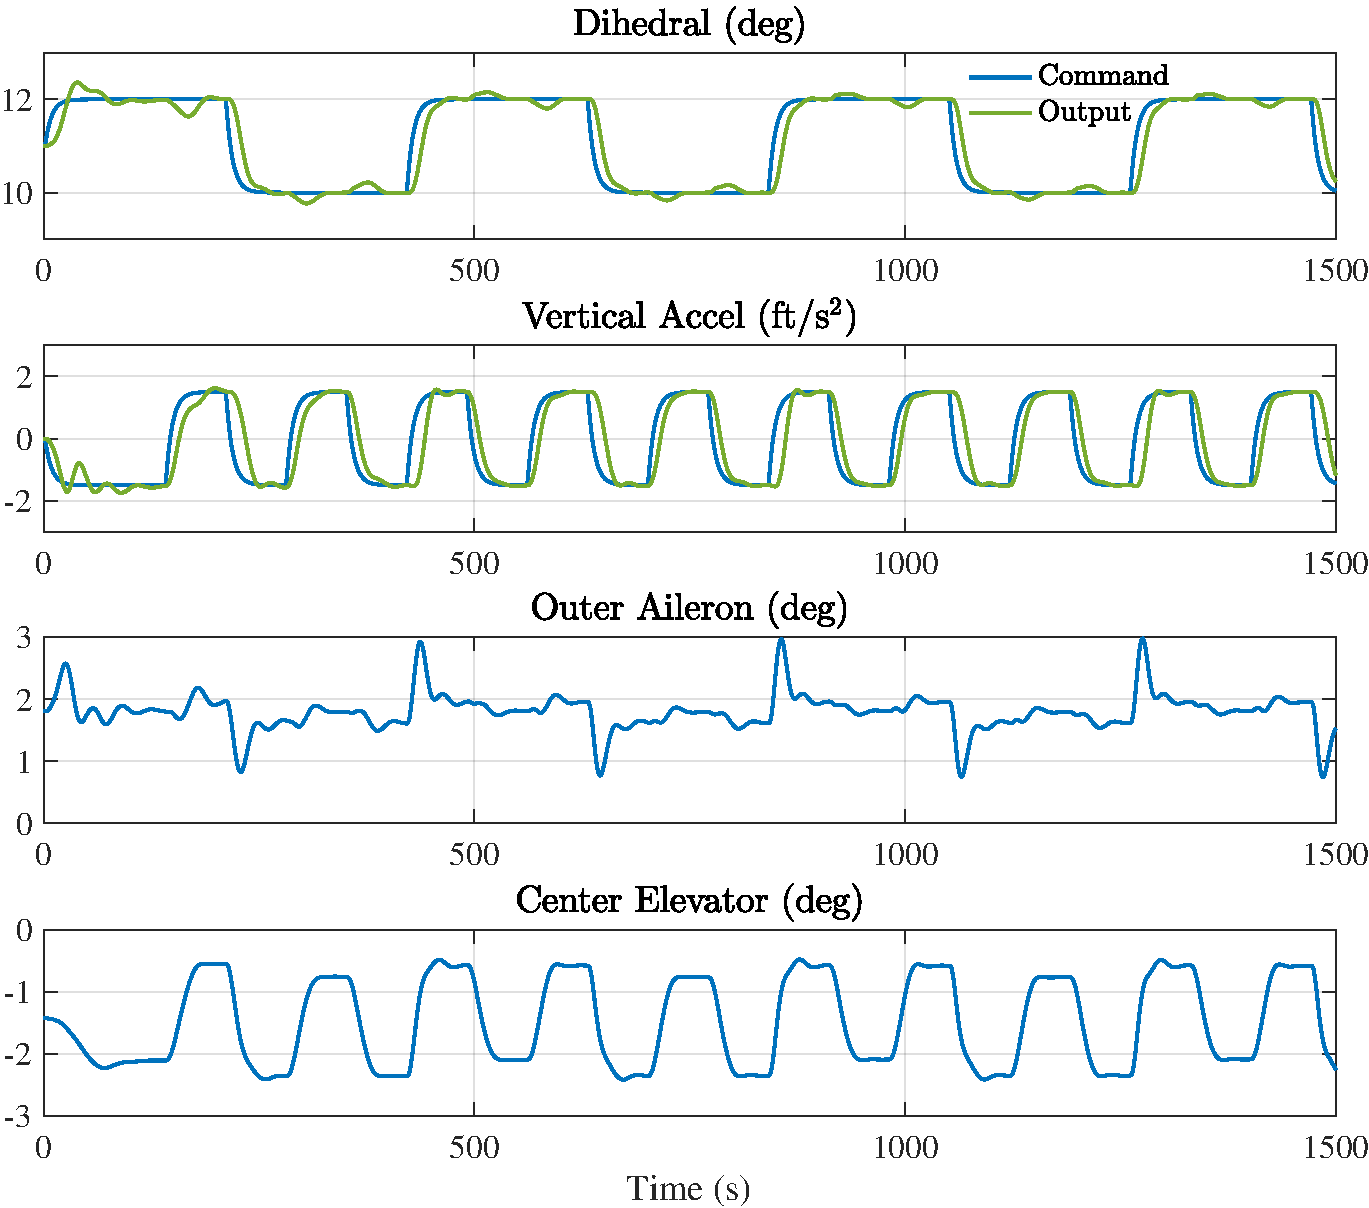
\includegraphics[width=\columnwidth]{../fig/nom3.pdf}
	\caption{Nom-3 simulation: RSLQR + MRAC with uncertainties $\Theta_p$, $\Lambda_p$, and $\Theta_1$}
	\label{fig:nom3}
\end{figure}

These simulations, presented in Figs. \ref{fig:nom1}, \ref{fig:nom2}, and \ref{fig:nom3} respectively, show how the MRAC controller with output feedback described in (\ref{eq:rd2-b1a})--(\ref{eq:rd2-adaptation}) is able to recover the desired closed-loop performance with uncertainty in plant and actuator parameters. With the baseline RSLQR controller only, the system suffers degraded command tracking performance in the presence of uncertainty (Fig. \ref{fig:nom2}), especially for vertical acceleration tracking.

We now simulate the introduction of a severe anomaly into the dynamics, causing the actuator dynamics to change suddenly from the uncertain first-order dynamics (\ref{eq:first_order_act}) to the uncertain second-order dynamics (\ref{eq:second_order_act}). The three responses to this anomaly which we will consider are
\begin{description}
	\item[AR-1 (Passive)] The RSLQR+MRAC autopilot retains control without intervention from the remote human supervisor
	\item[AR-2 (Manual)] The human operator takes over manual control of the affected vehicle
	\item[AR-3 (Shared)] Responsibilities are shared between the human pilot and autopilot as described in Section \ref{sec:shared_ctrl}
\end{description}

In these simulations, the vehicle operates in nominal operation with the RSLQR+MRAC control design for $0 \leq t < t_1^*$. At $t_1^* = 600 s$, the vehicle's actuators change from first-order (\ref{eq:first_order_act}) to second-order (\ref{eq:second_order_act}). Figs. \ref{fig:ar1}--\ref{fig:ar1-err} show the result of a passive response (AR-1) in which the human operator ignores vehicle performance degradation and allows the adaptive controller to continue operating on the plant with severely anomalous dynamics. The closed-loop system loses stability, leading to oscillations in vehicle output and eventual structural failure of the VFA at $t_3^* = 960 s$, 6 minutes after the introduction of second-order actuator dynamics. Note that a passive response using only the RSLQR controller (no MRAC) also leads to structural failure following the anomaly.

\begin{figure}[htbp]
	\centering
	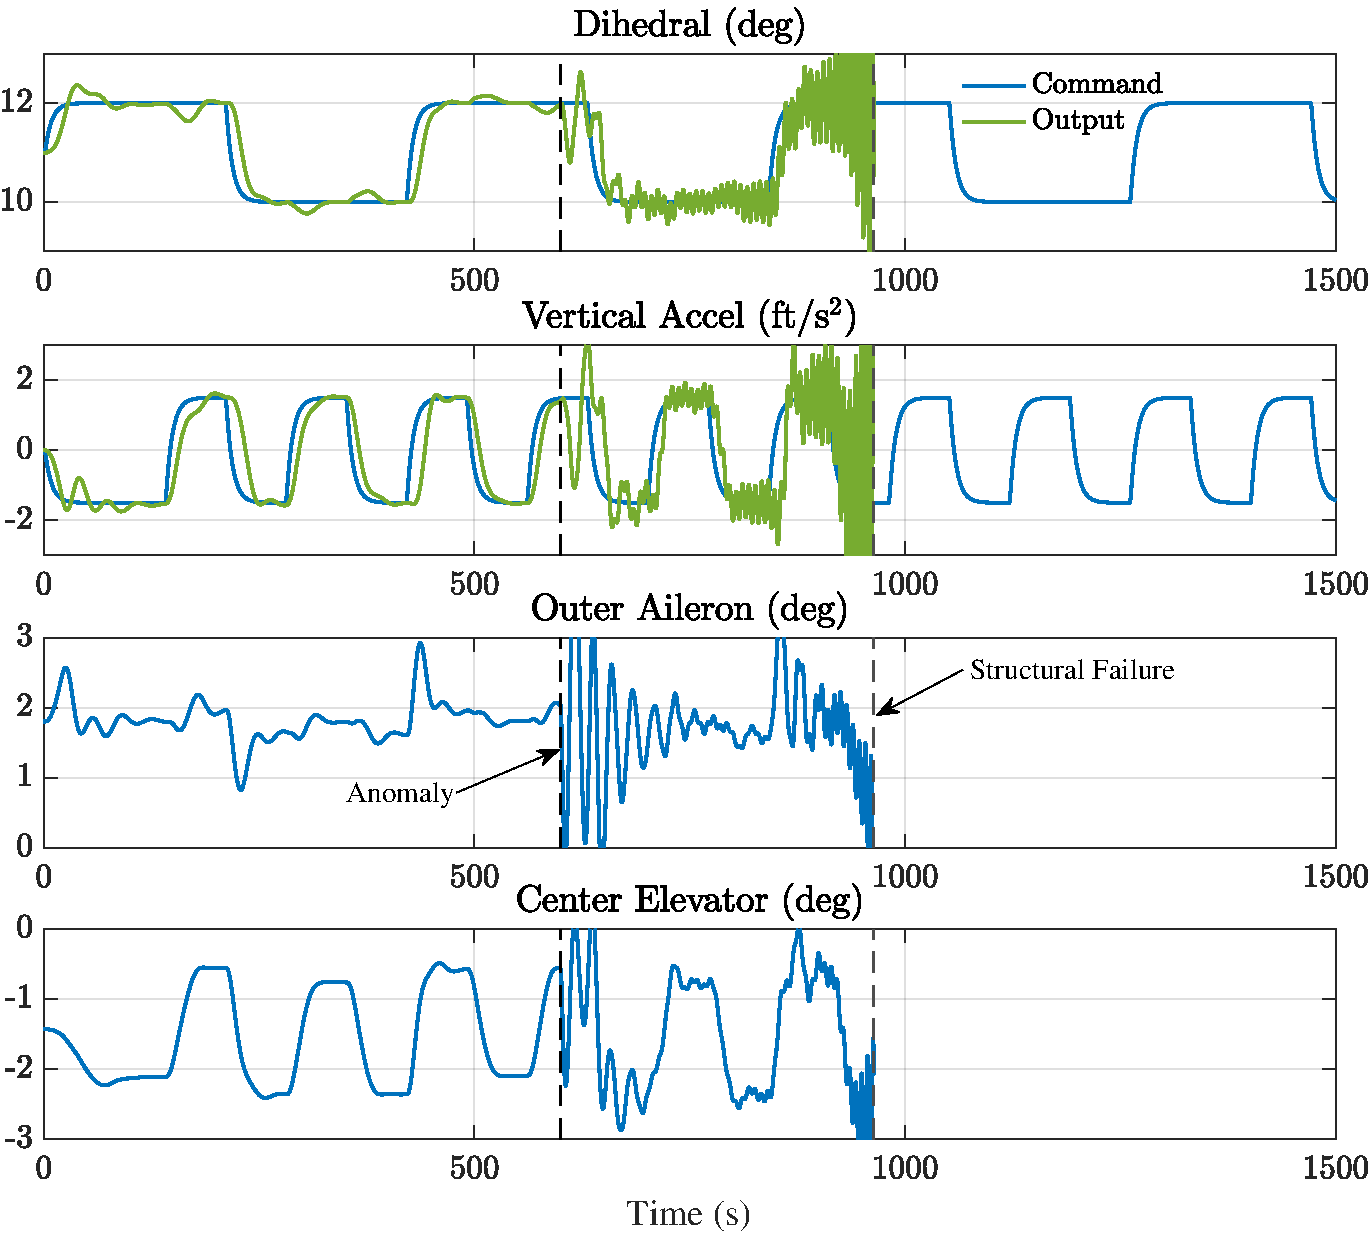
\includegraphics[width=\columnwidth]{../fig/ar1.pdf}
	\caption{AR-1 simulation: passive response to dynamical anomaly results in structural failure after 6 minutes}
	\label{fig:ar1}
\end{figure}

\begin{figure}[htbp]
	\centering
	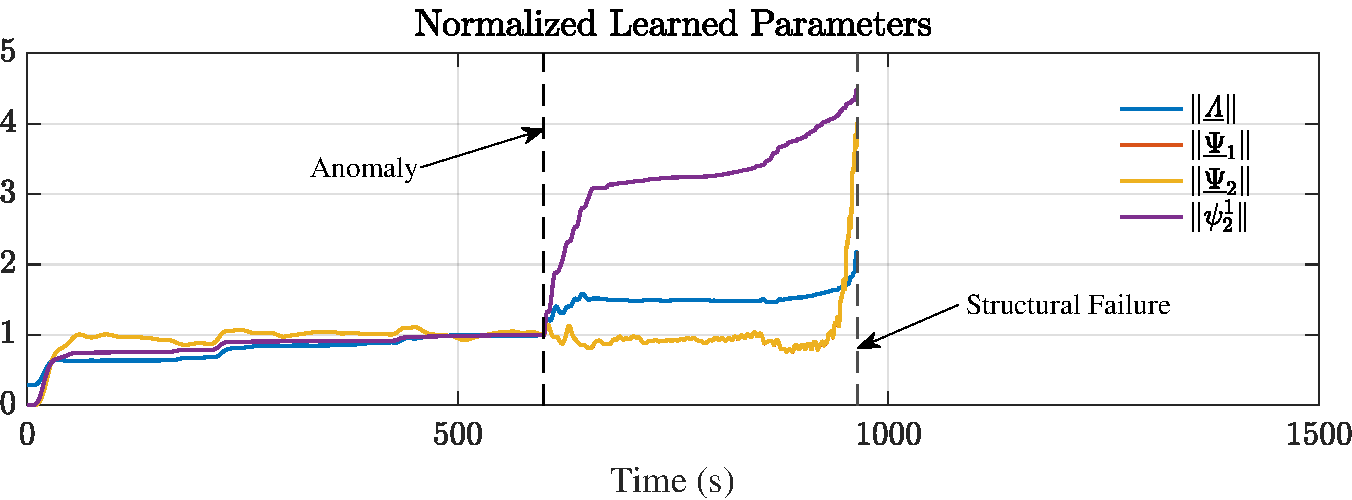
\includegraphics[width=\columnwidth]{../fig/ar1-params.pdf}
	\caption{AR-1 simulation: adaptive parameters diverge as controller struggles to adapt to unmodeled dynamics}
	\label{fig:ar1-params}
\end{figure}

\begin{figure}[htbp]
	\centering
	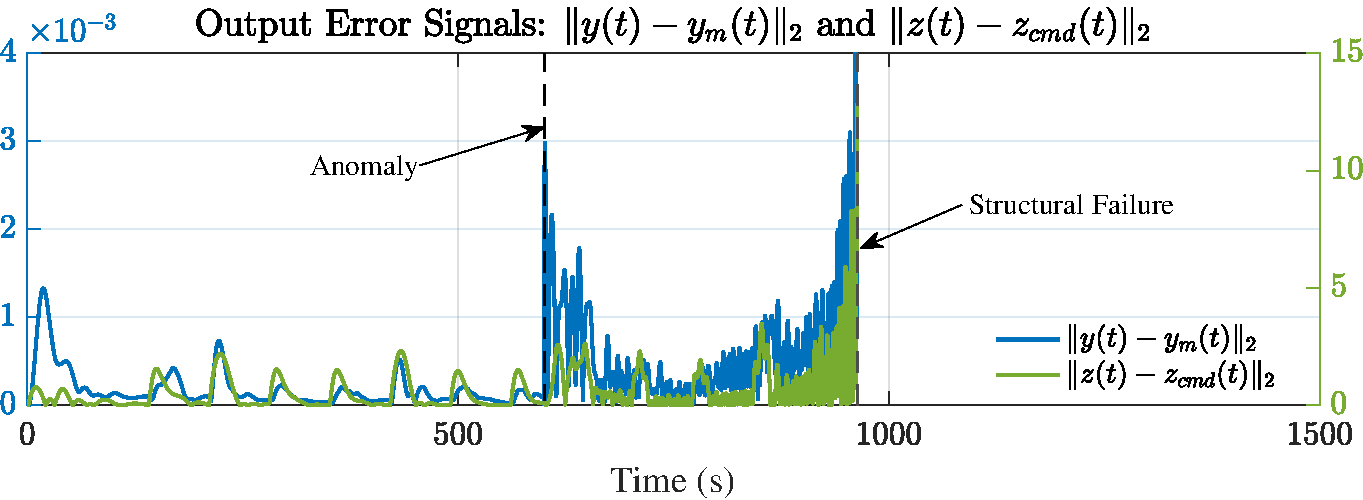
\includegraphics[width=\columnwidth]{../fig/ar1-err.pdf}
	\caption{AR-1 simulation: model-following output error and command tracking error grow after anomaly}
	\label{fig:ar1-err}
\end{figure}

Numerical simulations of the AR-2 response (purely manual control) are not carried out, as they are not deterministic and require high-fidelity \textit{human-in-the-loop} experiments to characterize. The limitations of such a response -- in which the human operator's role changes suddenly from ``on-the-loop'' to ``in-the-loop'' with unfamiliar dynamics -- are discussed in the earlier sections of this paper.

Results of the AR-3 (shared control) anomaly response simulation are shown in Figs. \ref{fig:ar3-sim}--\ref{fig:ar3-err}. After the anomaly is introduced at $t_1^* = 600 s$, the ``nominal'' controller attempts to control the system whose dynamics are not fully accounted for in the control model. Simultaneously in the shared control framework, the human operator notices the anomalous closed-loop control behavior, and via an interface switches the controller to the higher relative degree design (\ref{eq:rd3-b1a})--(\ref{eq:rd3-adaptation-deriv}) at $t_2^* = 800 s$, which is the culmination of the human operator's action. For $t \geq t_2^*$, the vehicle remains under autonomous control with the ``recovery'' adaptive controller and is able to reestablish nominal command tracking performance. For comparison, the time of structural failure in the passive anomaly response is plotted as a line at $t_3^* = 960 s$.

\begin{figure}[htbp]
	\centering
	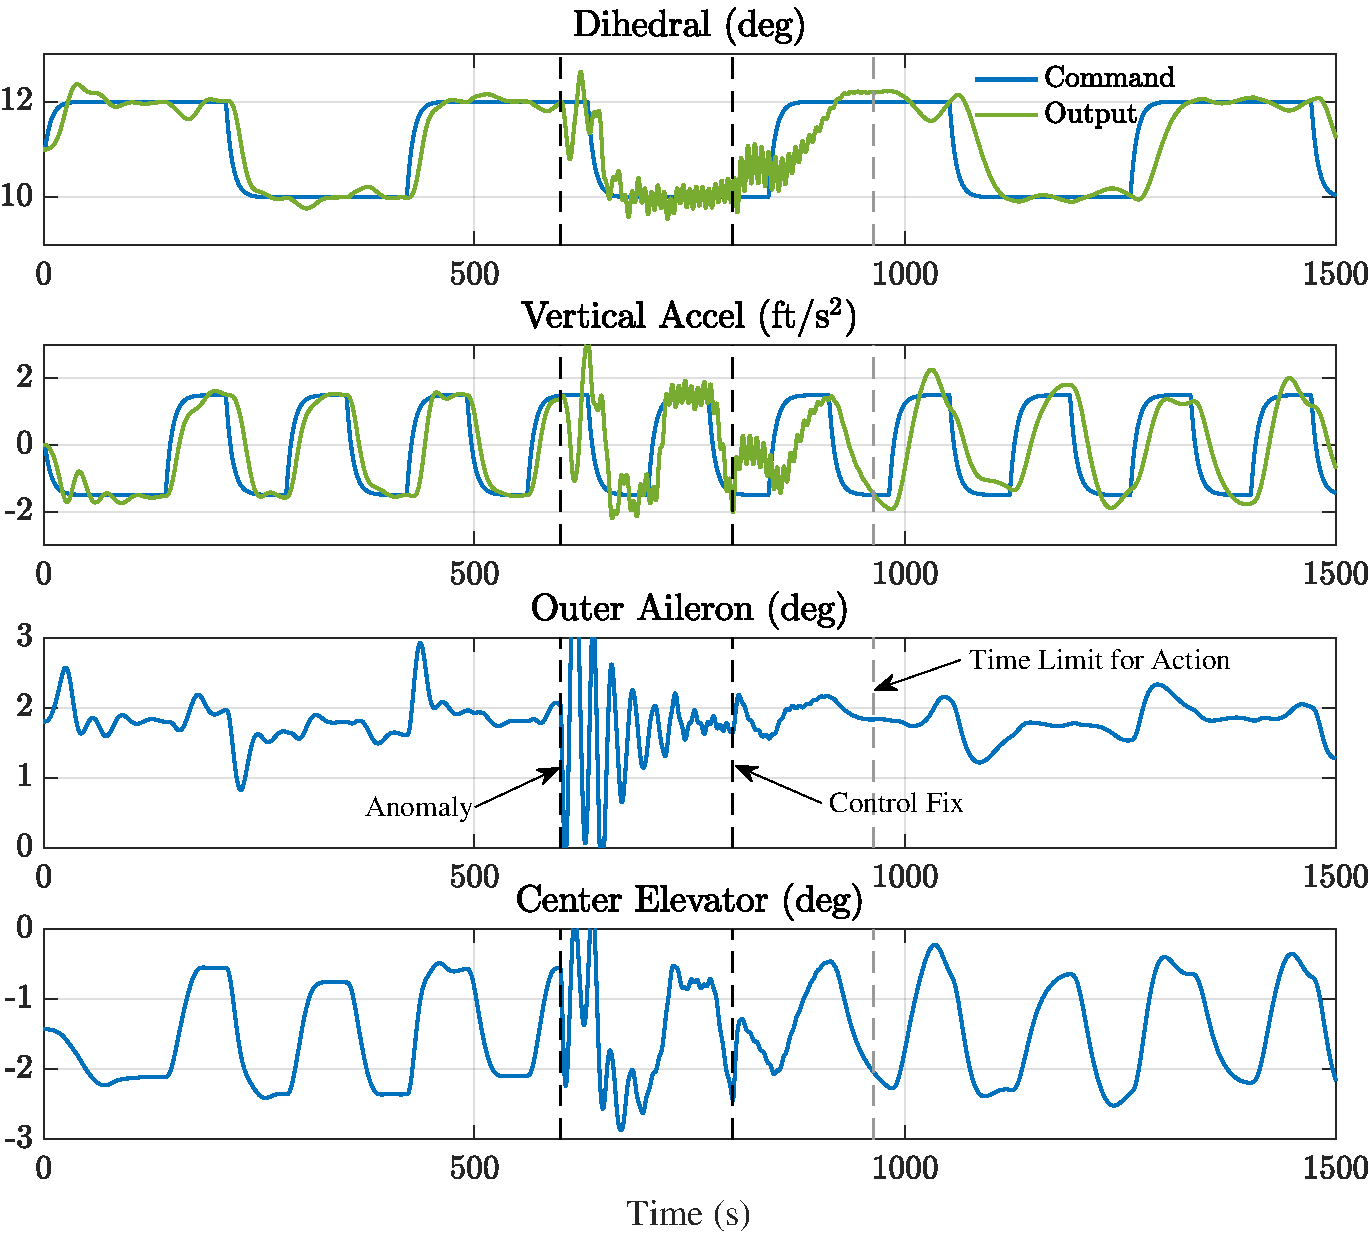
\includegraphics[width=\columnwidth]{../fig/ar3.pdf}
	\caption{AR-3 simulation: shared response to the dynamical anomaly results in recovery of vehicle performance}
	\label{fig:ar3-sim}
\end{figure}

\begin{figure}[htbp]
	\centering
	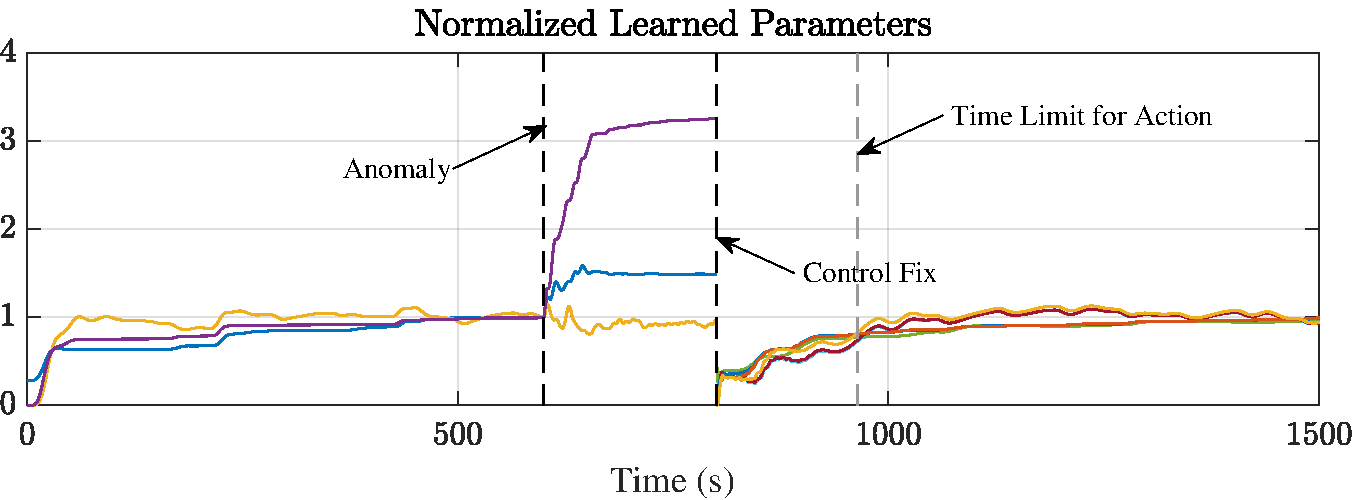
\includegraphics[width=\columnwidth]{../fig/ar3-params.pdf}
	\caption{AR-3 simulation: the change in control model at $t_2^* = 800 s$ stops the divergence of adaptive parameters}
	\label{fig:ar3-params}
\end{figure}

\begin{figure}[htbp]
	\centering
	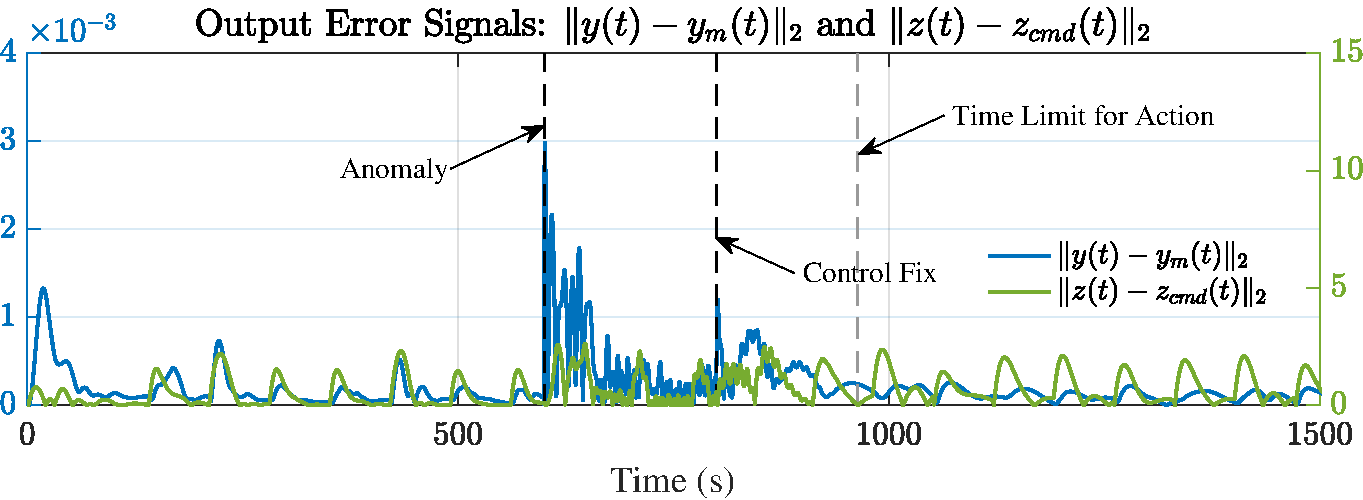
\includegraphics[width=\columnwidth]{../fig/ar3-err.pdf}
	\caption{AR-3 simulation: the change in control model at $t_2^* = 800 s$ returns error signals to nominal levels}
	\label{fig:ar3-err}
\end{figure}

\section{Summary}\label{sec:summary}
This work develops a shared control framework between adaptive autopilots and remote human operators of aerial vehicles. The autonomous control design builds on two recent advances in adaptive control theory, namely the use of closed-loop reference models for improved transient performance, and computationally efficient control designs for output-feedback systems having relative degree two or greater. In our shared response to dynamical anomalies, the human operator provides key inputs based on a higher-level perception of the anomaly, and these inputs are used by the adaptive autopilot retaining responsibility for low-level regulation and command tracking tasks. The shared control response is demonstrated in simulation on the longitudinal dynamics of an unmanned HALE VFA model. 

\bibliography{thomsen-cphs-2018-bib}

%\appendix
%\section{Passive RSLQR Anomaly Response}
%\begin{figure}[htbp]
%	\centering
%	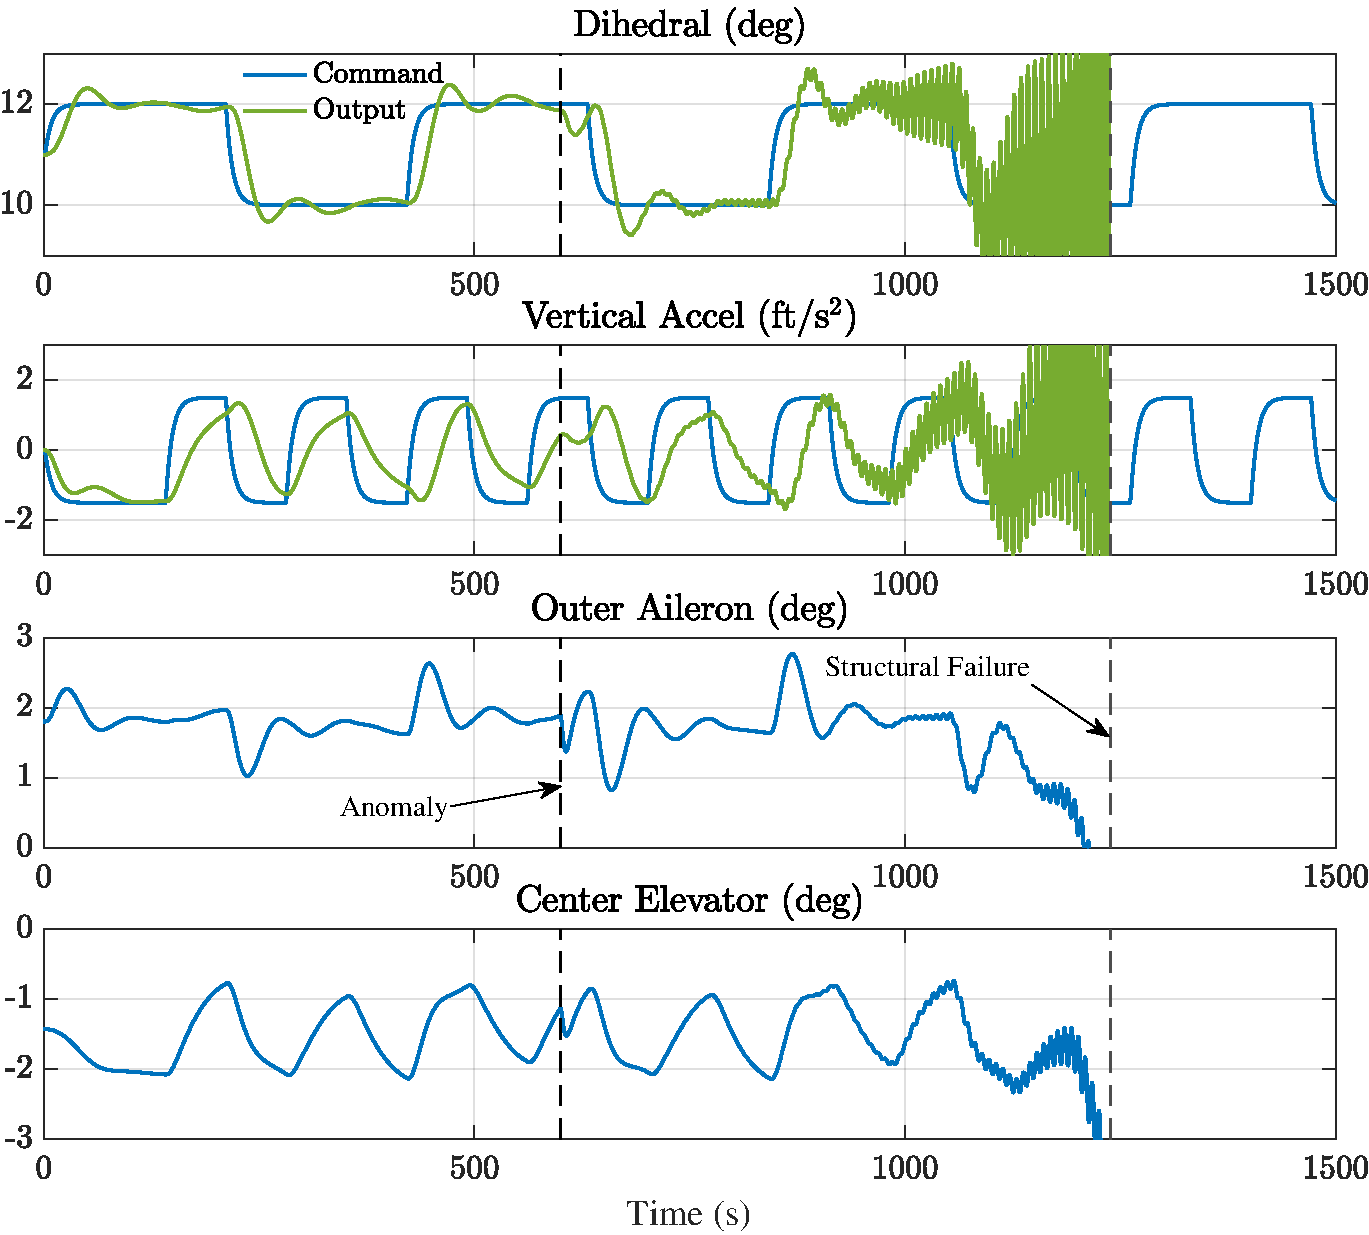
\includegraphics[width=\columnwidth]{../fig/ar-lqr.pdf}
%	\caption{AR-LQR simulation: The baseline RSLQR without MRAC becomes unstable after the introduction of an anomaly}
%	\label{fig:ar-lqr}
%\end{figure}
%
\end{document}
